\documentclass[
    a4paper,
    14pt,
    captions=tableheading,
    russian
]{scrreprt}

% Остальные стандартные настройки убраны в preamble.inc.tex.
%Package extsizes not only changes the fontsize, but also amends various skips as well as the margins.
%Changing the page geometry after loading the package will give fixed margins.
%\usepackage{extsizes}

%fonts and localization
\usepackage[utf8]{inputenc}
\usepackage{fontspec}
\RequirePackage{polyglossia}
\providehyphenmins{russian}{{3}{3}}
\setdefaultlanguage[babelshorthands=true,spelling=modern]{russian}
\setotherlanguage{english}
\setmainfont{Liberation Serif}
\setsansfont{Liberation Sans}
\setmonofont{Liberation Mono}
\newfontfamily\cyrillicfont{Liberation Serif}
\newfontfamily\cyrillicfontsf{Liberation Sans}
\newfontfamily\cyrillicfonttt[Scale=0.8]{Liberation Mono}
\defaultfontfeatures{Ligatures=TeX}
\defaultfontfeatures{Mapping=tex-text}

%math
\usepackage{amssymb}
\usepackage{amsmath}
%for \degree
\usepackage{gensymb}

% table of contents
\usepackage[tocflat]{tocstyle}

% bibliography
\usepackage[parentracker=true,
            backend=biber,
            language=auto,
            autolang=other,
            hyperref=auto,
            citestyle=gost-numeric,
            bibstyle=gost-numeric]
            {biblatex}
\DefineBibliographyStrings{russian}{
    bibliography = {Список использованных источников},
    references = {Список использованных источников}
}
\addbibresource{my.bib}
%disable uri encoding
\usepackage{hyperref}
\DeclareFieldFormat{url}{%
  \mkbibacro{URL}\addcolon\space
  \href{#1}{\nolinkurl{\thefield{urlraw}}}}

%setting page geometry
\usepackage[
a4paper, includefoot,
left=3cm, right=2cm, top=2cm, bottom=1.5cm,
headsep=1cm, footskip=1cm
]{geometry}

%not sure abt this
\usepackage{csquotes}
%quotations
\usepackage[
    left = «,%
    right = »,%
    leftsub = „,%
    rightsub = “%
]{dirtytalk}

%use \input for files. used with latexmk
\newcommand\inputfile[1]{%
    \InputIfFileExists{#1}{}{\typeout{No file #1.}}%
}

% line spacing
\usepackage[nodisplayskipstretch]{setspace}
\setstretch{1.5}

%pictures
\usepackage{graphicx}
\graphicspath{{img/}}
\DeclareGraphicsExtensions{.png,.jpg,.gif}

% \includepdf
\usepackage{pdfpages}

%disable hyphenation
%\disablehyphenation

%justifying
\usepackage{ragged2e}

%paragraph indent
\setlength{\parindent}{1.25cm}
\usepackage{indentfirst}

%titles
\newcommand*{\justifyheading}{\centering}
\usepackage[explicit]{titlesec}

\titleformat{\chapter}[display]
  {\normalfont\justifyheading\bfseries}
  {\thechapter}{1em}{\MakeUppercase{#1}}
  \titlespacing*{\chapter}{\parindent}{-18pt plus 4pt minus 2pt}{30pt plus 4pt minus 2pt}

\titleformat{\section}
  {\normalfont\bfseries}
  {\thesection}{1em}{#1}
  \titlespacing*{\section}{\parindent}{12pt plus 4pt minus 2pt}{12pt plus 4pt minus 2pt}

\titleformat{\subsection}
  {\normalfont\bfseries}
  {\thesubsection}{1em}{#1}
  \titlespacing*{\subsection}{\parindent}{12pt plus 4pt minus 2pt}{12pt plus 4pt minus 2pt}

\titleformat{\subsubsection}
  {\normalfont}
  {\thesubsubsection}{1em}{#1}
  \titlespacing*{\subsubsection}{\parindent}{12pt plus 4pt minus 2pt}{12pt plus 4pt minus 2pt}

%setting numeration
\renewcommand\thesection{\arabic{section}}
\renewcommand\thesubsection{\thesection.\arabic{subsection}}
\renewcommand\thesubsubsection{\thesubsection.\arabic{subsubsection}}
\setcounter{secnumdepth}{3}

%setting lists margin
\usepackage{enumitem}
%\setlist{nosep,leftmargin=\parindent}
\setlist{left=0pt .. \parindent,nosep}
%\setlist{labelindent=\parindent,leftmargin=*,nosep}

\usepackage{float}
%itemize separator
\renewcommand{\labelitemi}{—}
\renewcommand{\labelitemii}{—}
\renewcommand{\labelitemiii}{—}

\usepackage{chngcntr}
\counterwithin{equation}{section}
%tables and figures https://habr.com/ru/post/144648/
\usepackage[
    singlelinecheck=false, %for caption to be aligned left
    tableposition=top,
    figurewithin=section,tablewithin=section] %see chngcntr below
{caption}
\usepackage{subcaption}
\DeclareCaptionLabelFormat{gostfigure}{Рисунок #2}
\DeclareCaptionLabelFormat{gosttable}{Таблица #2}
\DeclareCaptionLabelSeparator{gost}{~—~}
\DeclareCaptionLabelFormat{continued}{Продолжение таблицы~#2}
\captionsetup{labelsep=gost}
\captionsetup[figure]{justification=centering,labelformat=gostfigure}
\captionsetup[table]{justification=raggedright,labelformat=gosttable}

\renewcommand{\thefigure}{\thesection.\arabic{figure}}
\renewcommand{\thesubfigure}{\asbuk{subfigure}}
\renewcommand{\thetable}{\thesection.\arabic{table}}
\renewcommand{\theequation}{\thesection.\arabic{equation}}

%\usepackage[notindex,nottoc]{tocbibind}

\usepackage{array, multirow, makecell}
\usepackage{pgfplotstable}
\usepackage{booktabs}

\usepackage{xtab}
\usepackage{etoolbox}
\makeatletter
\patchcmd{\estimate@lineht}{1\p@}{-2.5\p@}{}{}
\makeatother
% в \tablefirsthead{\shrinkheight{-\normalbaselineskip}}

\usepackage{paracol}
\setcellgapes{4pt}
\makegapedcells

\emergencystretch=15pt

\usepackage{verbatim}
\usepackage{desclist}


\begin{document}
% Some dirty hacks to stretch document
\tabulinesep=5pt% table rows spacing

\newdimen\origiwspc%
\newdimen\origiwstr%
\origiwspc=\fontdimen2\font% original inter word space
\origiwstr=\fontdimen3\font% original inter word stretch
\fontdimen3\font=1.6\origiwstr% (original) inter word stretch
\fontdimen2\font=0.4em% inter word space

\setlength{\emergencystretch}{70pt}

%\begin{center}
    \MakeUppercase{Министерство рогов и копыт}\\
    Федеральное государственное бюджетное образовательное учреждение
    высшего образования \say{Университет Пушкина}\\
    Кафедра Колотушкина\\
    Учебная дисциплина \say{Конструирование конструкторов}\\
    \hfill\break
    \hfill\break
    \hfill\break
    \hfill\break
    \hfill\break
    Лабораторные работы\\
    Прикольные и полезные (нет)\\
    \hfill\break
    \hfill\break
\end{center}

%\hfill\begin{minipage}{0.5\linewidth}
\begin{flushright}
    Выполнил: студент\\
    Группа: группа \\
    \underline{\hspace{3cm}} \\
    Проверил: преподаватель\\
    \underline{\hspace{3cm}} \\
    \say{\underline{\hspace{1cm}}} \underline{\hspace{2cm}} \the\year\\
\end{flushright}
%\end{minipage}
\hfill\break
\hfill\break
\begin{center}
    Городок\\
    \the\year
\end{center}
\thispagestyle{empty} % выключаем отображение номера для этой страницы

% КОНЕЦ ТИТУЛЬНОГО ЛИСТА

\newpage

\chapter*{Реферат}

Майларов Д.А. Разработка сети кафедры на базе тонких клиентов/терминальных станций

Дипломная работа содержит:
\begin{enumerate}
    \item страниц: \pageref{LastPage}; 
    \item рисунков: \totalfigures;
    \item таблиц: \totaltables;
    \item приложений: 1.
\end{enumerate}

Ключевые слова: сеть, тонкий клиент, терминал, программно-аппаратный комплекс,
Raspberry Pi, Windows, SolidWorks, RDP.

В ходе выполнения дипломной работы была разработана сеть кафедры на базе тонких
клиентов.

Работа написана мной самостоятельно и не содержит неправомерных заимствований.

\hspace*{\fill} Майларов Д.А.

\thispagestyle{empty} % выключаем отображение номера для этой страницы
\setcounter{page}{6} % номер страницы реферата

\tableofcontents
\thispagestyle{empty} % выключаем отображение номера для этой страницы

\addcontentsline{toc}{chapter}{Определения и сокращения}
\chapter*{Определения и сокращения}

В настоящей выпускной квалификационной работе используются следующие термины, сокращения
и обозначения с соответствующими определениями:

%\renewcommand{\descriptionlabel}[1]{\hspace{\labelsep}{#1}}

\noindent
	\begin{desclist}{}{ \rm\hfill —}[ПО]
		\item[БД] база данных
        \item[Дистрибутив] форма распространения программного обеспечения
        \item[Локальная вычислительная сеть (ЛВС)] частная сеть, размещенная, как
            правило, в одном здании или на территории одной организации
		\item[ОС] операционная система
		\item[ПАК] программно-аппаратный комплекс
		\item[ПК] персональный компьютер
		\item[ПО] программное обеспечение
        \item[САПР] система автоматизированного проектирования
		\item[ТК] тонкий клиент, терминал, устройство терминального доступа
		\item[Ethernet] семейство технологий пакетной передачи данных между
	устройствами для компьютерных и промышленных сетей. Ethernet в основном
	описывается стандартами IEEE группы 802.3
        \item[Linux] семейство Unix-подобных операционных систем на базе ядра Linux,
            включающих тот или иной набор утилит и программ, и, возможно,
            другие компоненты. 
        \item[Local Area Network (LAN)] локальная вычислительная сеть
        \item[Remote Desktop Protocol (RDP)] протокол удаленного доступа, используемый в
            ОС семейства Windows.
	\end{desclist}


\addcontentsline{toc}{chapter}{Введение}
\chapter*{Введение}

С развитием вычислительной техники системные требования программного обеспечения
становятся все более высокими. За последнее время производительность компьютеров
значительно выросла, поэтому старые устройства уже не справляются с современными
программами, особенно с требовательными САПР, используемыми в учебном процессе
на кафедре КПРС.

Актуальность работы состоит в том, что новые версии таких САПР, как SolidWorks 2019 и
Altium Designer 19, неудовлетворительно работают на компьютерах кафедры.
При модернизации компьютерных классов есть
возможность использовать подход к организации сети, основанный на тонких клиентах —
терминальных станциях, которые подключаются к производительному серверу, на котором
производятся вычисления.

Целью выпускной квалификационной работы является разработка общевычислительного
многопользовательского программно-аппаратного комплекса (ПАК) на основе тонких клиентов.

Объектом исследования является вычислительный комплекс кафедры.

Предмет исследования — модернизация вычислительного комплекса.

Для достижения заданной цели были поставлены следующие задачи:

\begin{enumerate}
    \item Рассмотреть технологии организации вычислительных сетей
    \item Разработать проект программно-аппаратного комплекса
    \item Установить и настроить комплекс
    \item Проанализировать результаты работы
\end{enumerate}

Практическая значимость работы состоит в том, что вычислительный комплекс кафедры может
быть модернизирован в соответствии с выдвигаемыми в работе предложениям, по прописанным
пошаговым инструкциям.

В первой главе рассматриваются основные технологии организации вычислительных сетей.

Во второй главе разрабатывается проект ПАК, выбирается программное и аппаратное
обеспечение.

В третьей главе описывается процесс установки и настройки комплекса, разрабатывается
корпус для изделия.

В четвертой главе анализируются результаты работы, исследуется производительность и
экономическая эффективность, проводится анализ на устойчивость к внешним воздействиям.

В заключении формулируются выводы и предложения по использованию результатов работы.


\chapter{Обзор технологий организации вычислительных сетей}

\section{Определение локальных сетей}

Локальными сетями называют частные сети, размещающиеся, как правило, в одном здании или
на территории какой-либо организации. Их часто используют для объединения компьютеров и
рабочих станций в офисах компании или предприятия бытовой электроники для предоставления
совместного доступа к ресурсам (например, принтерам) и обмена информацией
\cite{tanenbaum}. Важными требованими, предъявляемыми к ЛВС, являются:

\begin{itemize}
    \item Низкий уровень ошибок передачи, вызванных внутренними или внешними факторами.
        Допустимая вероятность ошибок передачи данных должна быть порядка
        $10^{-8}$–$10^{-12}$.
    
    \item Возможность  работы  с  большими нагрузками  или высокая интенсивность обмена.
        Если механизм управления в сети не эффективен, то компьютеры могут подолгу ждать
        свою очередь на передачу. И даже если передача будет на высочайшей высоте и
        безошибочна, задержка доступа пользователю данной сети будет неприемлема.
\end{itemize}

Большинство ЛВС имеет выход в глобальную сеть. Но характер информации,  принципы
организации  обмена,  режимы  доступа  к  ресурсам внутри (ЛВС), как правило, отличаются
от принципов, принятых в глобальной сети. Возможность выхода в глобальную сеть — это
лишь один из ресурсов, разделяемых пользователями ЛВС. По ЛВС могут передаваться:
данные, изображения, телефонные разговоры, электронные письма и т.д. Чаще всего ЛВС
используются для совместного использования дискового пространства, принтеров и факсов,
выхода в глобальную сеть, но это лишь часть тех возможностей, которые предоставляют ЛВС. 

Например,  они  позволяют  осуществлять  обмен  информацией между
компьютерами  разных типов. ЛВС дают возможность организовать систему параллельных
вычислений на всех компьютерах сети, что ускоряет решение сложных задач. С их помощью,
можно управлять работой техноло-гической системы или исследовательской установки с
нескольких компью-теров одновременно. Однако ЛВС имеют ряд существенных недостатков:

\begin{itemize}
    \item ЛВС требует дополнительных, иногда значительных материальных затрат на
        покупку сетевого оборудования, ПО, на прокладку кабелей и обучение персонала. 
    \item ЛВС требует приема на работу специалиста (администратора сети),  который
        будет контролировать  работу сети, модернизировать, управлять доступом к
        ресурсам, устранять возможные неисправности, защищать информацию и делать
        резервные копии. Для больших сетей может понадобиться целая бригада
        специалистов. ЛВС ограничивает перемещение компьютеров, подключенных к ней, так
        как при этом требуется перекладка соединительных кабелей.
    \item ЛВС являются прекрасной средой для распространения компьютерных  вирусов,
        поэтому придется уделять  много  времени  вопросу о защите от них. Все
        компьютеры сети могут быть заражены, если заразить всего один.
    \item ЛВС резко повышают опасность несанкционированного доступа к информации с целью
        ее кражи или уничтожения. Информационная защита требует проведения комплекса
        технических и организационных мероприятий.
\end{itemize}

ЛВС классифицируются,  прежде  всего, по протоколам  1-го  и  2-го уровней OSI, то есть,
по технологии используемого сетевого оборудования: Ethernet, Token Ring, FDDI,
AppleTalk. По масштабам и иерархии построения ЛВС различают: 
\begin{itemize}
    \item сети рабочих групп (5-20 станций); 
    \item сети отделов (20-100 станций); 
    \item сети предприятий (корпоративные сети).
\end{itemize}

Последние имеют  развернутую структуру  сетевых  служб  и  по  географии могут выходить
за рамки локальных сетей, образуя кампусные сети, сети с удаленным доступом, а также
сети других масштабов, вплоть до корпоративных частных глобальных сетей. Количество
станций в корпоративных сетях варьируется: от 20 компьютеров до десятков тысяч.

\begin{figure}[h]
    \center
    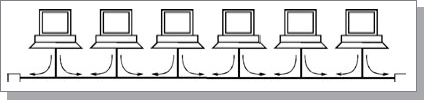
\includegraphics[width=0.7\linewidth]{topo_bus}
    \caption{Топология {шина}}
    \label{pic:topo_bus}
\end{figure}
\begin{figure}[h]
    \center
    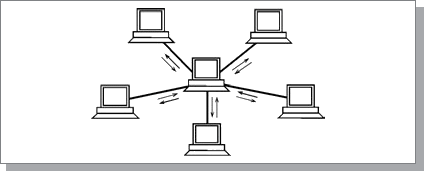
\includegraphics[width=0.7\linewidth]{topo_star}
    \caption{Топология {звезда}}
    \label{pic:topo_star}
\end{figure}
\begin{figure}[h]
    \center
    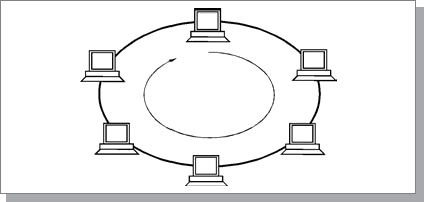
\includegraphics[width=0.7\linewidth]{topo_ring}
    \caption{Топология {кольцо}}
    \label{pic:topo_ring}
\end{figure}

Для организации сетей используются различные топологии. Основных топологии, применяемые
в ЛВС, такие: 

Шина (bus) — все устройства параллельно подключаются к одной линии связи. Информация
от каждого устройства одновременно передается всем остальным
(см. рисунок \ref{pic:topo_bus}).

Звезда (star) — к одному центральному устройству присоединяются остальные периферийные
устройства, причем каждый из них использует отдельную линию связи. Информация
от периферийного устройства направляется только центральному, а от него —
одному или нескольким периферийным
(см. рисунок \ref{pic:topo_star}).

Кольцо (ring) — устройства последовательно объединены в кольцо. Передача информации
в кольце всегда производится только в одном направлении. Каждое из устройств
передает информацию только одному следующему в цепочке за ним, а
получает информацию только от предыдущего в цепочке.
(см. рисунок \ref{pic:topo_ring}).

В зависимости от характера распределения функций различают: 

\begin{itemize}
    \item одноранговые  сети — небольшие  локальные  сети,  в которых компьютеры являются
        равноправными; обычно включают в себя до 15 станций;

    \item сети с выделенными серверами (двухранговые сети) — средние и крупные сети, в
        которых часть выполняемых функций обслуживания станций возложена на серверы. Такие
        сети характеризуются типами  используемых в них сетевых служб: файловая служба,
        служба печати, служба терминалов, управление базами данных, Web-служба, почтовая
        служба, службы интерактивного общения, прокси-сервер, сетевая безопасность.
\end{itemize}


\subsection{Архитектуры вычислительных сетей}

Вычислительные системы имеют два основных вида построения архитектуры: централизованный
и распределенный (также называемый клиент-сервер).

Основное различие между ними состоит в том, что в централизованной архитектуре большая
часть вычислений происходит на сервере. В распределенной системе все машины имеют
одинаковое назначение и все занимаются вычислениями.

Система клиент-сервер состоит из двух типов взаимодействующих устройств (см.
рисунок~\ref{pic:client-server}).
В большинстве случаев взаимодействие происходит по следующей модели:

\begin{enumerate}
    \item Клиент отправляет запрос на получение данных серверу;
    \item Сервер, получив запрос, начинает обработку данных, различные расчеты и т.п.
        (в зависимости от назначения сервера);
    \item Сервер отправляет обработанные или новые данные клиенту.
\end{enumerate}

\begin{figure}[h]
    \center
    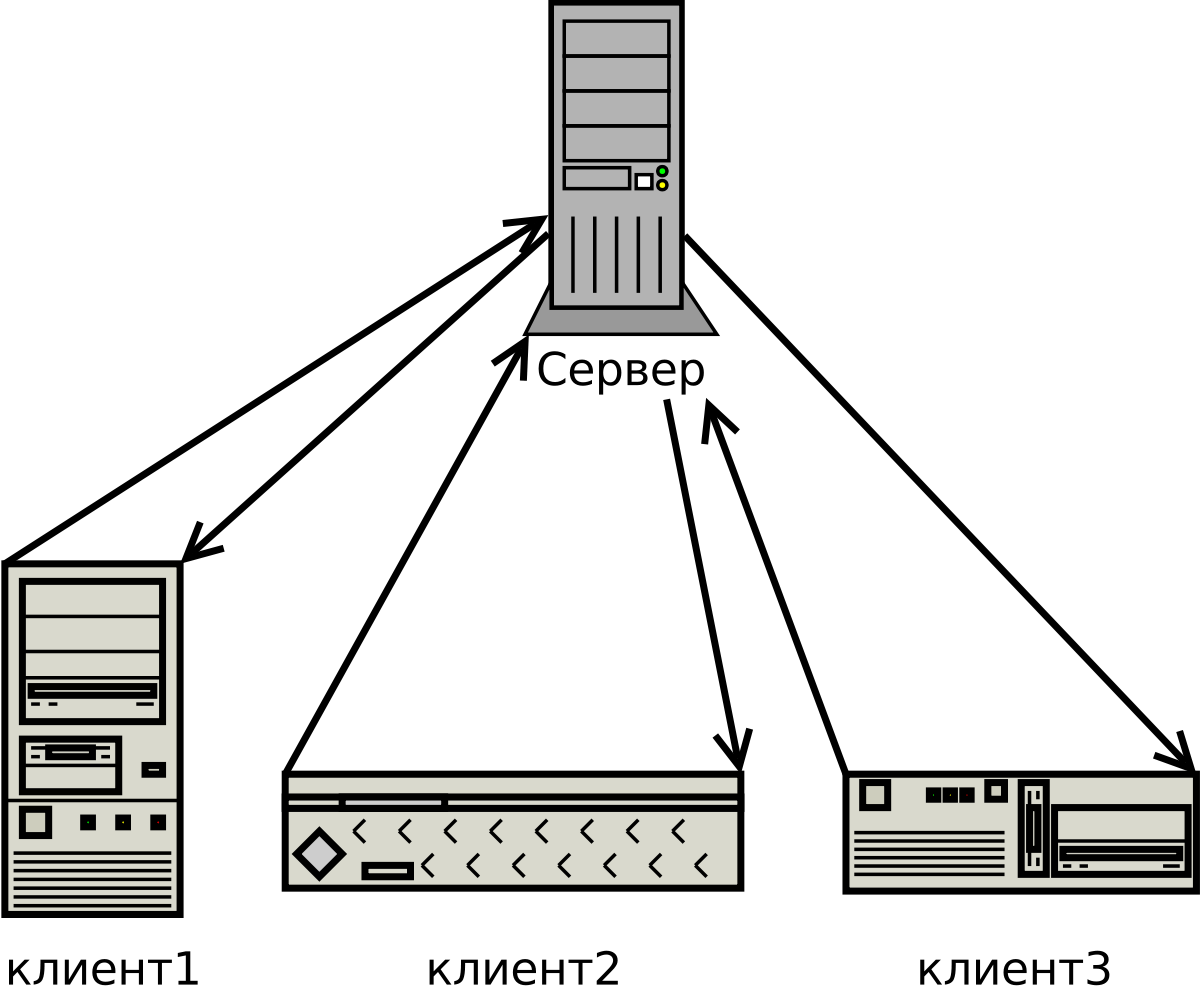
\includegraphics[height=9cm]{client-server}
    \caption{Клиент-серверная архитектура}
    \label{pic:client-server}
\end{figure}

\begin{figure}[h]
    \center
    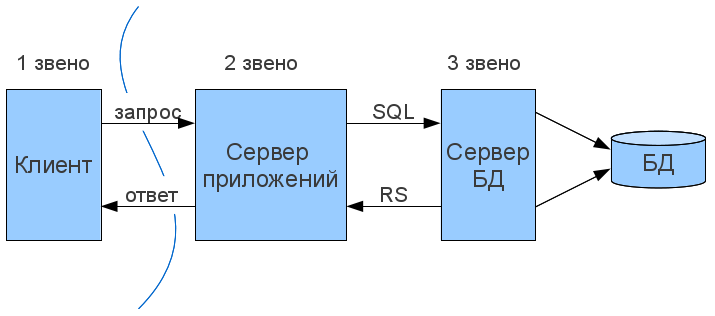
\includegraphics[height=5cm]{client-server-db}
    \caption{Клиент-серверная архитектура с разделением серверов}
    \label{pic:client-server-db}
\end{figure}

В настоящее время в сетях с централизованной архитектурой может быть применен принцип
разделения обязанностей серверов. Например, разделение серверов приложений, баз данных и
вычислений (см. рисунок~\ref{pic:client-server-db}).


\subsection{Терминальные системы}
Первые компьютеры 50-х годов предназначались для очень небольшого числа избранных
пользователей. Такие компьютеры не были предназначены для интерактивной работы
пользователя, а применялись в режиме пакетной обработки.  Задания нескольких
пользователей группировались в пакет, который принимался на выполнение. Распечатанные
результаты пользователи получали обычно только на следующий день.

По мере удешевления процессоров в начале 60-х годов появились новые способы организации
вычислительного процесса, которые позволили учесть интересы пользователей.  Начали
развиваться интерактивные многотерминальные системы разделения времени.  В таких
системах каждый пользователь получал собственный терминал, с помощью которого он мог
вести диалог с компьютером.
Действительно, рядовой пользователь работу за терминалом мэйнфрейма воспринимал примерно
так же, как сейчас он воспринимает работу за подключенным к сети персональным
компьютером. Пользователь мог получить доступ к общим файлам и периферийным устройствам,
при этом у него поддерживалась полная иллюзия единоличного владения компьютером, так как
он мог запустить нужную ему программу в любой момент и почти сразу же получить
результат. \cite{olifer}

Дальнейшее развитие информационных технологий и удешвление персональных компьютеров
привело к падению релевантности терминальных систем. Однако, в настоящее время тип
организации сетей, в основе которого лежат терминалы, называемые "тонкими клиентами" (в
противовес "толстым клиентам" — обычным ПК), вновь набирает популярность. Из-за
увеличения числа ПК в сетях их обслуживание становится все более сложным. Поэтому тонкие
клиенты стали снова широко использоваться.

\section{Система тонких клиентов}
Тонкий клиент, как и классический терминал 50–60-х годов, дает пользователю возможность
взаимодействия с удаленным компьютером. Разница в том, что если мощностей терминалов,
мэйнфреймов и пропускной способности сети хватало только для отправки текстовых команд и
получения текстовых результатов, то современные тонкие клиенты позволяют пользователям
взаимодействовать и с графическими интерефейсами, работать с графикой и даже
воспроизводить видео. Для пользователя тонкого клиента взаимодействие с удаленным
рабочим столом должно выглядеть неотличимо от обычного ПК. Современные ТК позволяют это
сделать.

Система, основанная на тонких клиентах, состоит из терминального сервера и одного и
более ТК. На терминальном сервере установлена ОС, позволяющая подключение ТК. Все
клиенты настроены на подключение к этому серверу и занимаются только вводом-выводом
информации для взаимодействия с пользователем, и выполнением протоколов удаленного
доступа. Все вычисления, работа ОС и процессов, взаимодействие с устройствами хранения
информации выполняются на сервере. 

Таким образом, все ресурсоемкие процессы в системе ТК перенесены на сервер. Это
означает, что для клиентских машин нужно минимальное аппаратное обеспечение, достаточное
для вывода изображения на экран, работы с сетью и устройствами ввода-вывода. В качестве
таких клиентов могут выступать как специализированные устройства, так и устаревшие ПК,
мощности которых уже не хватает для привычных пользователям задач.
(см. рисунок~\ref{pic:PCtoTC}).

\begin{figure}[htpb]
    \center
    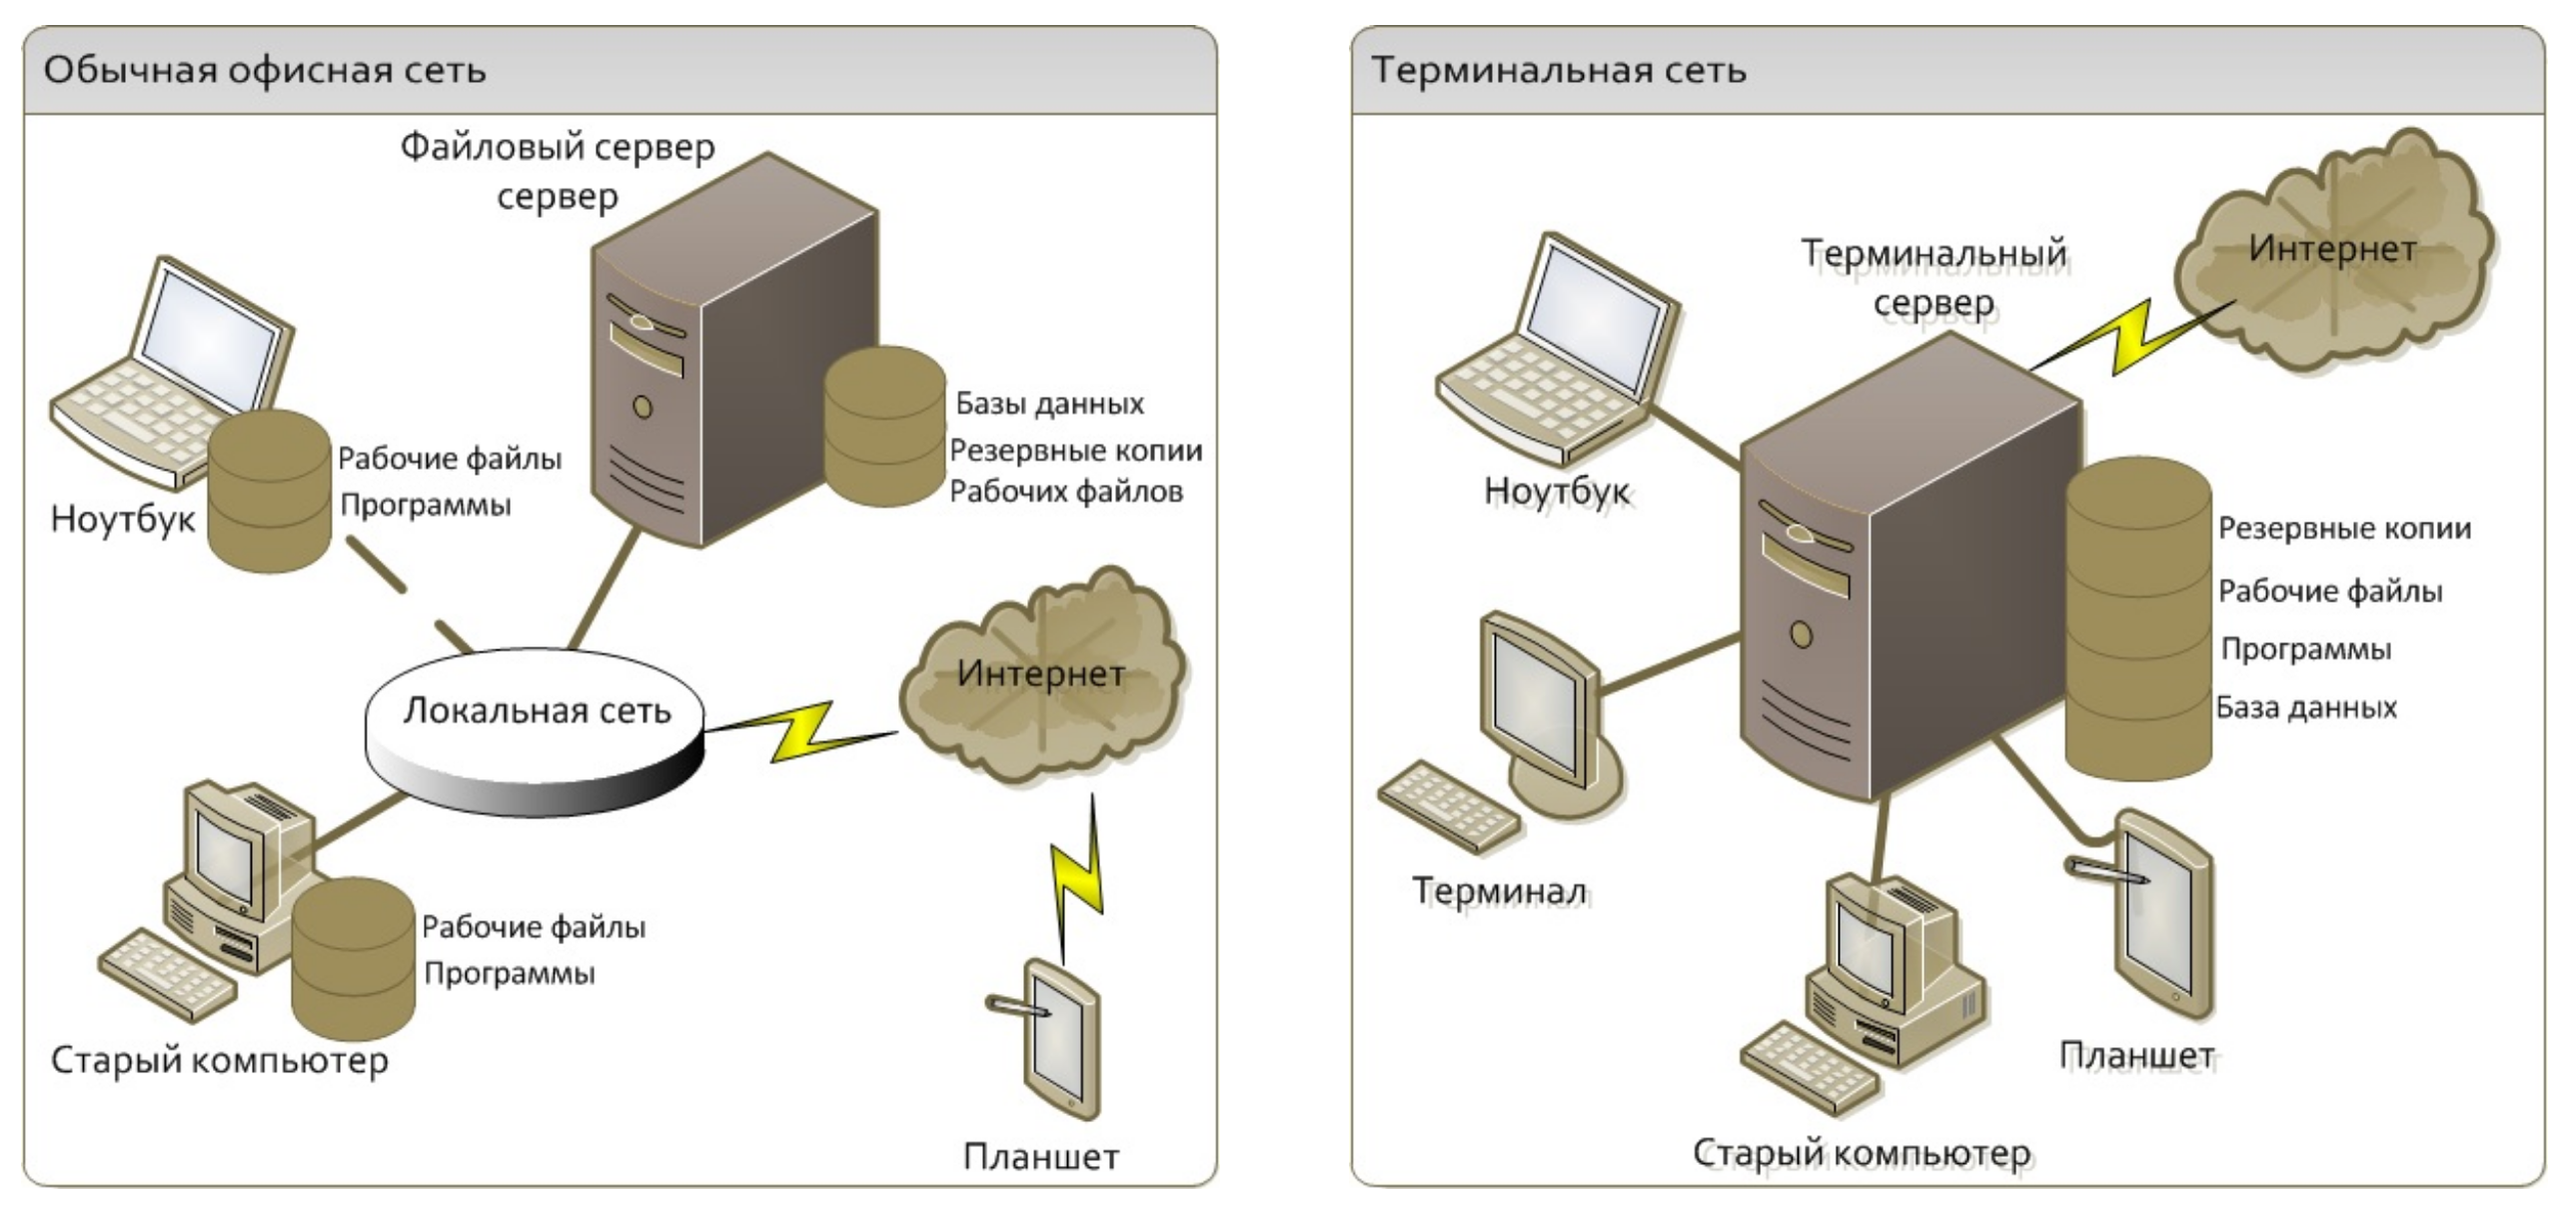
\includegraphics[width=\linewidth]{PCtoTC}
    \caption{Сравнение типовой и терминальной сетей. Источник: \cite{PCtoTCsrc}}
    \label{pic:PCtoTC}
\end{figure}

Преимущества систем, построенных на базе тонких клиентов:
\begin{itemize}
    \item   Экономия средств. Необходимость в постоянной модернизации всего парка
        компьютеров с выходом более новых и ресурсоёмких ОС и приложений исчезает.
        Модернизировать, при необходимости, нужно будет только терминальный сервер и
        серверы БД; терминалы не нуждаются в модернизации в течение длительного времени
        (7-10 лет). Лицензия терминального доступа стоит дешевле настольной ОС, не нужны
        локальные антивирусы, сложное ПО управления парком ПК, что значительно сокращает
        затраты. Снижается количество рутинных операций, а также перемещений IT
        персонала для обслуживания подразделений. При использовании терминала нет
        необходимости дополнительно приобретать источник бесперебойного питания для
        защиты от внезапного отключения питания, вся информация остается доступной на
        серверах. Даже при аппаратной замене ТК пользователь может продолжить работу.
    \item   Надежность. Использование серверной операционной системы и аппаратуры
        сервера повышает надежность работы и хранения данных. Выход из строя терминала,
        его утрата не повлекут за собой потерю или порчу данных на сервере.
    \item   Безопасность. Отсутствие на клиентских машинах жестких дисков, дисководов и
        приводов оптических дисков позволяет избежать несанкционированного копирования и
        выноса данных. Отсутствие непосредственной передачи данных по сети позволяет
        избежать их перехвата. Все программное обеспечение ставится только системным
        администратором. При краже или изъятии обычного компьютера есть риск потерять
        важные конфиденциальные данные, хранящиеся на нем. Терминал гораздо менее
        привлекателен для воров, т.к. не применим в домашних условиях, а при
        использовании тонких клиентов данные на конечном устройстве не хранятся.
    \item   Централизация. Все данные хранятся только на серверах, что упрощает
        процедуру резервного копирования, контроля версий ПО, контроля доступа
        пользователей. Всё ПО находится на серверах - это упрощает администрирование.
        Конечный пользователь не может повлиять на стабильность такой системы.
    \item   Эффективность. Загрузка процессора на ПК в большинстве случаев не превышает
        4-5\%. Терминальная система позволяет максимально полезно использовать
        вычислительные ресурсы сервера, распределяя их между работающими в данный момент
        пользователями.
    \item   Снижение энергопотребления. Тонкие клиенты используют
        энергоэффективные процессоры и не имеют подвижных компонентов, потребляют всего
        около 10\% мощности обычного ПК.
    \item   Тихая работа. Из-за низкого энергопотребления тепловыделение процессоров ТК
        невелико. Это позволяет использовать активные систмы охлаждения с малыми
        скоростями вращения вентиляторов, или использовать полностью пассивные системы
        охлаждения, что обеспечивает бесшумную работу клиентов.
    \item   Быстрое развертывание и обновление приложений. При использовании ТК вы
        просто устанавливаете новое ПО на серверах, и оно становится доступным сотням
        пользователей сразу после публикации.
    \item   Устранение поддержки конечных узлов. ПК – источник аппаратных проблем и
        проблем локальных конфигураций. При использовании ТК отпадает необходимость
        подходить к пользовательским устройствам для настройки системы, установки и
        ремонта программ, помощи в настройке приложений, замены сломанных деталей. ТК
        используют операционную систему терминального сервера, а приложения
        устанавливаются на серверах. Служба техподдержки может помогать пользователям
        посредством удаленного управления их терминальными сеансами. При выходе ТК из
        строя его легко заменить, что может выполнить специально назначенный сотрудник,
        даже не имеющий IT образования.
    \item   Защита от вирусов. Тонкие клиенты не подвержены заражению вирусами, на них
        антивирусное ПО не устанавливается. Достаточно установить антивирусное ПО на
        серверы компании. Локальный ПК не защищен от заражения при сбое параметров
        обновления или настройки антивируса и дальнейшего распространения вируса в ИС.
\end{itemize}

Из существенных недостатков системы на базе ТК можно выделить только необходимость
первоначальной настройки системы. Для внедрения данной системы нужно подготовить
достаточно производительный терминальный сервер, а также настроить его в соответствии с
планируемой архитектурой сети.  Также для корректной работы всей сети администратор
должен знать о ее организации.  Требуется более высокая квалификация администратора,
т.к. в его обязанности также будет входить поддержка протоколов удаленного доступа,
использованных в системе.  Однако, это компенсируется более низкой требуемой
квалификацией техников.

\subsection{Постановка задачи на разработку}

На момент разработки на кафедре КПРС имеется ЛВС, построенная по классической
одноранговой топологии \say{звезда}. Каждое рабочее место, подключенное к сети, является
полноценным \say{толстым клиентом}. Сеть используется только для предоставления доступа
к Интернет. Прочие сетевые технологии (такие как общий файловый сервер) практически не
используются. Исходя из этого, можно выделить задачи на разработку:

\begin{enumerate}
    \item Необходимо модернизировать сеть кафедры для обеспечения возможности
        совместного доступа к ресурсам сети и создания выделенного компьютера,
        выполняющего роль сервера рабочих столов.
    \item Разработать экономически целесообразное устройство, используемое в качестве
        тонкого клиента.
    \item Заменить часть рабочих мест на тонкие клиенты.
\end{enumerate}

Для выполнения этих задач было принято решение создать на базе существующей сети
программно-аппаратный комплекс, включающий в себя сервер терминалов, тонкие клиенты и
сеть, соединяющую их для совместного доступа к ресурсам. Требования к ПАК приведены в
таблице~\ref{tab:reqs}.

\begin{table}[h]
    \centering
    \caption{Технические требования к комплексу}
    \label{tab:reqs}
    \begin{tabularx}{\linewidth}{Xr}
        \toprule
        Технология канального уровня & Ethernet \\
        Количество подключенных рабочих мест, от & 3 \\
        Пропускная способность, Гбит & 10 \\
        \midrule
        Возможность многопользовательского доступа & SolidWorks \\
                                                   & Altium Designer \\
                                                   & OrCAD PCB \\
                                                   & и т.п. \\
        \midrule
        Масштабируемость & \\
        Экономическая эффективность & \\
        Экологичность и энергоэффективность & \\
        \multicolumn{2}{l}{Возможность постепенной модернизации} \\
        \multicolumn{2}{l}{Максимальное использование имеющегося аппаратного
        обеспечения} \\
        \bottomrule
    \end{tabularx}
\end{table}


\section{Разработка программно-аппаратного комплекса}

\subsection{Серверная аппаратная часть}
Для выбора серверной аппаратной части нужно опираться, в первую очередь, на системные
требования используемого на кафедре ПО. Для оценки в таблице \ref{tab:solid_req}
приводятся системные требования основного используемого на кафедре КПРС САПР SolidWorks
с сайта разработчика Dassault Systems \cite{ref:solid_req2} \cite{ref:solid_req1}.

\begin{table}[htpb]
    \centering
    \caption{Системные требования Solidworks}
    \label{tab:solid_req}
    \begin{tabu}to \linewidth{Xr}
        \toprule
        Процессор & 3.3 ГГц или выше \\
        RAM & 16 ГБ или более \\
            & 32 ГБ рекомендуется для Simulation \\
            & и работы с большими сборками \\
        Устройство хранения & рекомендуется SSD \\
        Место на диске & 20 ГБ и более \\
        \bottomrule
    \end{tabu}
\end{table}

\begin{table}[htpb]
    \centering
    \caption{Характеристики сервера}
    \label{tab:srv_spec}
    \begin{tabu}to \linewidth{Xr}
        \toprule
        Процессор & AMD Ryzen 5 2600 \\
        Видеокарта & AMD Radeon RX 570 4GB \\
        Частота процессора & 3.8 ГГц \\
        Количество потоков & 12 \\
        Объем RAM & 16 ГБ \\
        Частота RAM & DDR4, 3200 МГц \\
        Устройство хранения & 1ТБ SSD \\
        \bottomrule
    \end{tabu}
\end{table}

Требования для многопользовательской работы не указаны, поэтому нужно провести
дополнительные исследования производительности системы при многопользовательской работе.
По предварительным испытаниям компьютер кафедры обеспечивает достаточную
производительность для базовой работы в Soldiworks двух подключенных клиентов.

В связи со сложной эпидемиологической ситуацией, доступ к реальным компьютерам на
кафедре затруднен. Для тестирования в качетстве сервера будет применяться компьютер на
базе процессора AMD Ryzen 5 2600. Его характеристики приведены в
таблице~\ref{tab:srv_spec}.

\subsection{Клиентская аппаратная часть}
Для работы в качестве тонкого клиента подходит практически любой x86-совместимый
компьютер, на котором есть возможность запустить клиент нужного протокола.
Соответственно, существующие на кафедре компьютеры могут быть использованы в качестве
ТК. Однако, для получения многих преимуществ ТК есть смысл использовать более
компактные и энергоэффективные системы.

В качестве основной платформы для разработки ТК будет использован одноплатный компьютер
Raspberry Pi 3B. Его характеристики приведены в таблице \ref{tab:rpi_specs}, внешний вид
— на рисунке \ref{pic:piphoto}.

\begin{table}[h]
    \centering
    \caption{Технические характеристики Raspberry Pi 3B}
    \label{tab:rpi_specs}
    \begin{tabu}to \linewidth{Xr}
        \toprule
        Процессор & однокристальный чип Broadcom BCM2837 \\
        микроархитектура & ARM Cortex-A53 \\
        разрядность & 64-бит \\
        количество ядер & 4 \\
        тактовая частота & 1,2 ГГц \\
        оперативная память & 1ГБ LPDDR2 SDRAM \\
        \midrule
        цифровой видеовыход & HDMI \\
        композитный выход & 3,5 мм (4 pin) \\
        USB порты & USB 2.0×4 \\
        сеть & WiFi 802.11n, 10/100 Мб RJ45 Ethernet \\
        Bluetooth & Bluetooth 4.1, Bluetooth Low Energy \\
        разъем дисплея & Display Serial Interface (DSI) \\
        разъем видеокамеры & MIPI Camera Serial Interface (CSI-2) \\
        карта памяти & MicroSD \\
        порты ввода-вывода & 40 \\
        габариты & 85x56x17 мм \\
        \bottomrule
    \end{tabu}
\end{table}

\begin{figure}[h]
    \center
    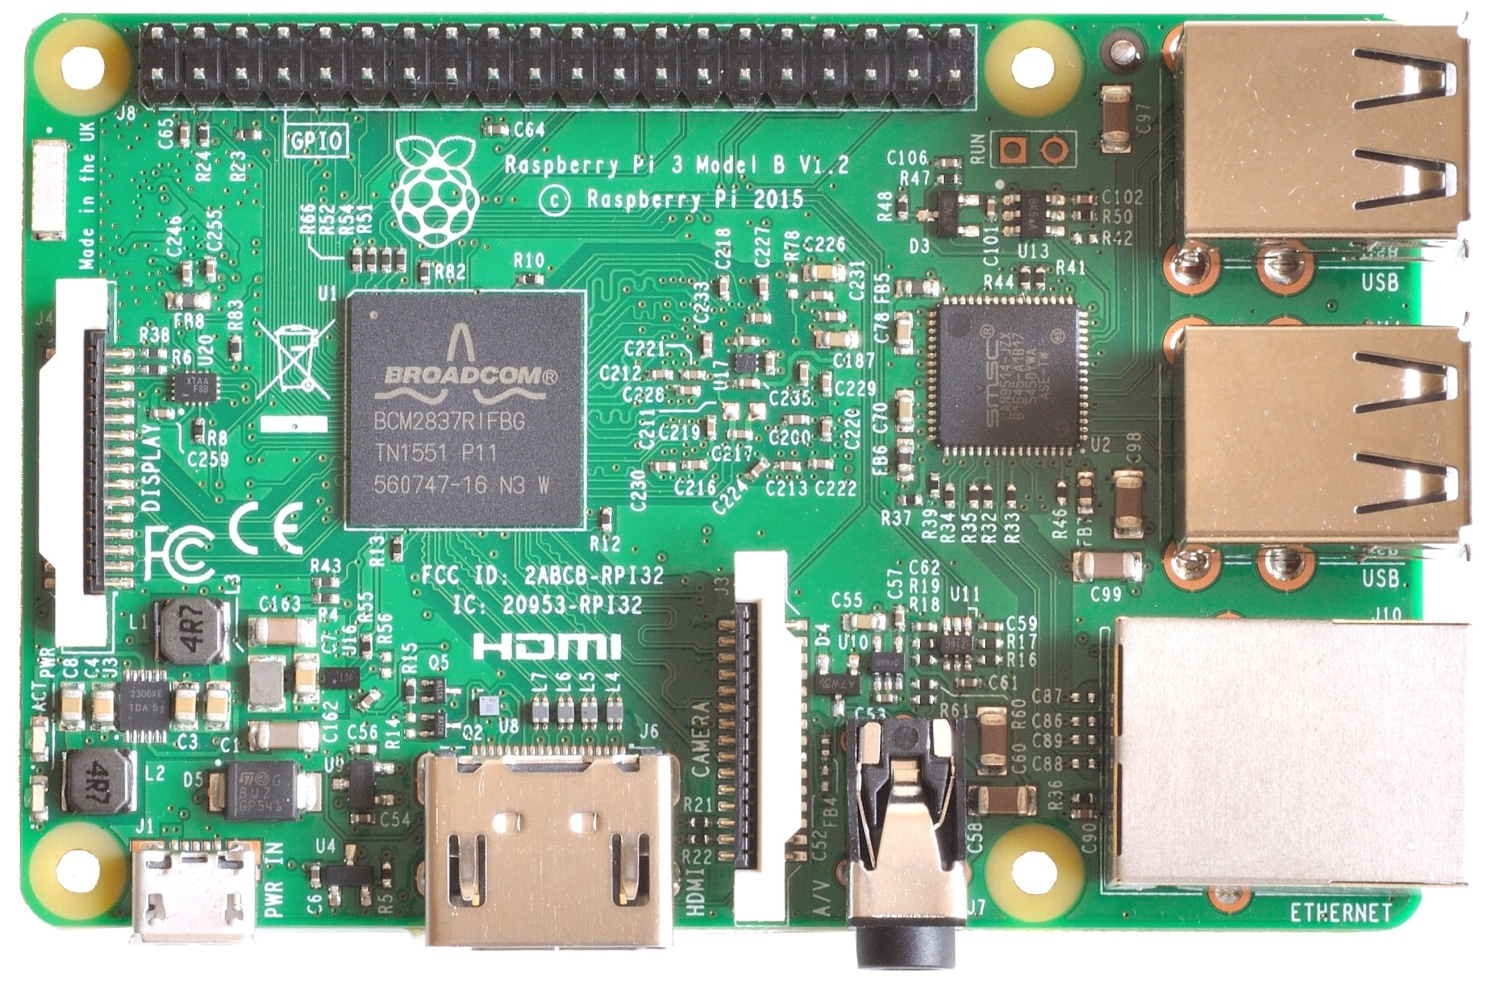
\includegraphics[width=\linewidth]{piphoto}
    \caption{Внешний вид Raspberry Pi 3B}
    \label{pic:piphoto}
\end{figure}

К недостаткам такого решения относятся:
\begin{itemize}
    \item Отсутствие в комплекте поставки корпуса, блока питания, SD-карты.
    \item Невозможность использования аппаратного ускорения графики, т.к. отсутствуют 
        драйвера с открытым исходным кодом для BCM2837.
    \item Производительность зависит от нагрева процессора, необходимость качественного
        охлаждения.
    \item ARM архитектура снижает количество доступного ПО (по сравнению с
        x86-совместимыми устройствами).
\end{itemize}

Стоит отметить, что эти недостатки будут частично устранены при разработке данного
проекта.
По результатам предварительных исследований, производительности Raspberry Pi 3B
достаточно для использования в этом проекте.

\subsection{Серверное ПО и лицензирование}

Для работы программных пакетов, представленных в задании на разработку, необходима ОС
семейства Windows. Также, необходима ОС, позволяющая многопользовательскую работу, то
есть Windows Server. Актуальная на момент разработки версия — Windows Server 2019. У
данной версии есть три варианта: Essentials, Standart и Datacenter.
\cite{ref:win_srv_overview}\cite{ref:win_srv_comp}.

\begin{table}[h]
    \centering
    \caption{Сравнение редакций Windows Server 2019}
    \label{tab:win_srv_comp}
    \begin{tabu}to \linewidth{X[1,c,m]X[1,c,m]X[1,c,m]X[1,c,m]}
        \toprule
        Редакция & Essentials & Standart & Datacenter \\
        \midrule
        Лицензирование & На сервер & На ядро + CAL & На ядро + CAL \\
        Виртуализация & Да & Да; 2~виртуальные
        машины и один узел Hyper-V на лицензию & Да; неограниченное количество
        виртуальных машин и один узел Hyper-V на лицензию. \\
        Защищенные виртуальные машины & Нет & Нет & Да \\
        Программные сетевые интерфейсы & Нет & Нет & Да \\
        Программное хранилище данных & Нет & Нет & Да \\
        \bottomrule
    \end{tabu}
\end{table}

\begin{enumerate}
    \item Datacenter ‒ предназначен для развёртывания в облачных средах и в центрах по
        обработке данных при высоком уровне виртуализации. Лицензия приобретается по
        принципу: одна лицензия \say{на ядро} (core-based);
    \item Standard ‒ ориентирована для использования в среде с минимальными уровнями
        виртуализации, а также в физической среде. Лицензирование производится так же,
        как и в случае с \say{Datacenter};
    \item Essentials ‒ редакция, ориентированная на малый бизнес, с ограничением на
        количество клиентов — допускается не более 50 устройств и максимум 25
        пользователей. Данная редакция получает лицензию по методу server-based:
        один физический сервер – одна лицензия (на каждый дополнительный сервер
        необходимо приобретать новую лицензию).
\end{enumerate}

Подробное сравнение этих вариантов приводится в таблице~\ref{tab:win_srv_comp}.
Также стоит отметить, что для многопользовательской работы в редакциях Standart и
Datacenter необходимо покупать дополнительные лицензии для каждого клиента. Такие
лицензии называются Client Activation License (CAL).

Исходя из этих ограничений, можно выбрать редакцию Essentials для разрабатываемого
проекта. Ограничения касаются в основном функций виртуализации, которые в данном проекте
не используются.

\subsection{Выбор используемого протокола}

Для разработки необходимо выбрать способ удаленного доступа, который будет
использоваться в системе. Так как выбор зависит от серверной ОС, выбор оптимального
варианта связан с доступными на Windows протоколами.

Основной протокол, используемый в Windows — RDP (Remote Desktop Protocol). Клиент RDP
доступен во всех редакциях Windows, начиная с Windows XP, что позволяет использовать
любой компьютер кафедры в качестве тонкого клиента (см. рисунок \ref{pic:mstsc_xp}).
Однако, RDP-клиенты существуют для многих платформ, в том числе для Linux.

Актуальные версии протокола RDP:
\begin{itemize}
    \item Версия 6.0 установлена в Windows Vista и включила поддержку программ
        удаленного взаимодействия, приложениям Windows Presentation Foundation,
        поддержку нескольких мониторов и поддержку большого рабочего стола. Эта версия
        доступна для Windows XP с пакетом обновления (SP2), Windows Server 2003 SP1 /
        SP2 (выпуски x86 и x64) и Windows XP Professional x64 Edition. Microsoft Remote
        Desktop Connection для Macintosh OS X также доступен с поддержкой Intel и
        PowerPC Mac OS версии 10.4.9 и выше.
        
    \item Версия 6.1 была выпущена в феврале 2007 и включена в Windows Server 2008, и в
        пакет обновления Windows Vista SP1 и Windows XP SP3.  В дополнение к изменениям,
        связанным с улучшенным доступом к консоли, эта версия включает новые
        функциональные возможности, появившиеся в Windows Server 2008, такие как
        Terminal Services Easy Print driver (новая клиентская система перенаправления
        принтера, которая позволяет выполнять локальную печать из приложений,
        выполняющихся на сервере, не устанавливая драйвер печати на сервере).
    \item Версия 7 (вышла в составе Windows 7, поддерживается в Windows XP). Особенности
        этой версии:
    \begin{itemize}
        \item Поддержка аутентификации сетевого уровня (NLA), что снижает риск успешной
            атаки типа отказ в обслуживании (DoS);
        \item Увеличение производительности ядра RDP;
        \item Поддержка технологии Windows Aero (Aero over Remote Desktop);
        \item Поддержка технологий Direct2D и Direct3D 10.1 в приложениях;
        \item Полноценная поддержка мультидисплейных конфигураций;
        \item Улучшения в работе с мультимедиа;
        \item Поддержка технологии Media Foundation;
        \item Поддержка технологии DirectShow;
        \item Снижена длительность задержки при воспроизведении аудио.
    \end{itemize}

    \item Версия 7.1 (вышла в составе Windows 7 SP1);
    \item Версия 8.0 (вышла в составе Windows 8, с октября 2012 года доступна как пакет
        обновления для Windows 7 SP1 и Windows Server 2008);
    \item Версия 8.1 (вышла в составе Windows 8.1, с ноября 2013 года доступна как пакет
        обновления для Windows 7 SP1 и Windows Server 2008 R2);
    \item Версия 10 (Вышла в составе Windows 10, с 29 июля 2015 года. Последней версией
        является 10.0.16299.15, входящей в состав Windows 10 1809. Десятая версия
        включает в себя ряд новых функций, например, масштабирование AutoSize (полезно
        для клиентов HiDPI). Улучшен алгоритм сжатия графики с использованием H.264/AVC.
\end{itemize}

Используемая версия протокола RDP — 10, последняя на данный момент, т.к. используется
актуальная версия Windows Server.

\subsection{Клиентское ПО}

В качестве клиентской ОС выбран стандартный для Raspberry Pi дистрибутив Linux Raspbian,
основанный на Debian \cite{ref:raspbian}.
Дистрибутив поддерживается Raspberry Pi Foundation и рекомендован к установке.
К его преимуществам можно отнести открытый исходный код, простоту установки и удобство 
настройки. 
Актуальной на момент разработки была версия Buster, вышедшая в феврале 2020 года.

При загрузке ОС пользователь будет попадать в менеджер окон Openbox. Он настроен на
автоматический запуск RDP-клиента, также в случае необходимости (например, для
устранения проблем с сетевым подключением) его можно будет настроить для работы в режиме
обычного ПК, то есть как \say{толстый клиент}.

Для RDP-клиента использовано ПО FreeRDP, актуальной на момент разработки версии 2.0.0
\cite{ref:freerdp}. Данный программный продукт позволяет осуществлять подключение к
RDP-серверам любой версии, просто и гибко настраивается для получения оптимальной
производительности.  Так как исходный код открыт, есть возможность скомпилировать
бинарный файл для нужной архитектуры (в рассматриваемом проекте используется архитектура
ARM).

Так как FreeRDP не имеет графического интерфейса, для запуска будет использован скрипт,
выполняющийся при загрузке системы и позволяющий сразу подключиться к серверу. 

\begin{figure}[p]
    \center
    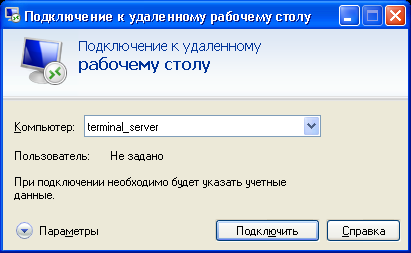
\includegraphics[height=8cm]{mstsc_xp}
    \caption{Окно RDP-клиента, встроенного в Windows XP}
    \label{pic:mstsc_xp}
\end{figure}

\begin{figure}[p]
    \center
    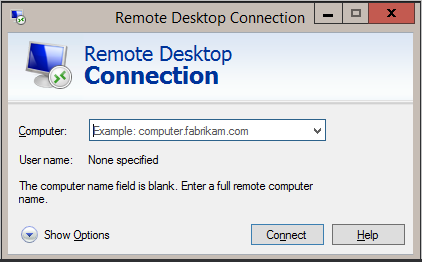
\includegraphics[height=8cm]{mstsc_10}
    \caption{Окно RDP-клиента, встроенного в Windows 10}
    \label{pic:mstsc_10}
\end{figure}

Также при необходимости подключения Windows-клиентов может быть использован встроенный в
систему RDP-клиент (см. рисунки~\ref{pic:mstsc_xp},~\ref{pic:mstsc_10}). Это может быть
полезным, в том числе, для подключения личных ноутбуков студентов или уже имеющихся ПК
с ОС Windows.

\subsection{Корпус тонкого клиента}

Как указано выше, микрокомпьютер Raspberry Pi поставляется без корпуса. Соответственно,
требуется разработать конструкцию для защиты платы от внешних воздействий. Конструкция
не должна препятствовать охлаждению системы, иначе возникнут проблемы с
производительностью.

Так как плата Raspberry Pi является достаточно популярной, для нее существуют различные
варианты корпусов, как официальные, так и модели от сторонних производителей. Для
разработки нужно проанализировать имеющиеся варианты.

\begin{enumerate}
    \item Корпус Waveshare Electronics 11619 \cite{ref:case_oval}. Корпус выполнен из
        черного пластика, состоит из двух пластин и задней стенки с перфорацией.
        Пластины скрепляются саморезами, 4 шт. Задняя стенка устанавливается в пазы.
        Стоимость: 630 рублей.

        Корпус изображен на рисунке~\ref{pic:case_oval}.
        Так как приток холодного воздуха к SoC не обеспечен, есть опасность перегрева
        чипа. Данный корпус использовался на этапе тестирования сетевой части изделия.

    \item Корпус Waveshare Electronics 11655 \cite{ref:case_off}. Официальный корпус от
        Raspberry Pi Foundation. Корпус выполнен из пяти пластиковых частей со съемными
        крышкой и боковыми частями белого цвета.  Обеспечивает быстрый доступ к портам
        камеры и дисплея, а так же разъему расширения HAT. Предусмотрена съемная боковая
        часть для удобного доступа к 40-контактному порту GPIO.
        Стоимость: 810 рублей.

        Корпус изображен на рисунке~\ref{pic:case_oval}.
        Корпус обеспечивает охлаждение чипа только при снятии верхней крышки, при этом
        отсутствует защита платы от механических повреждений. Также возможность снятия
        боковых частей является излишней.
        
    \item Корпус Seeed Studio 114990129 \cite{ref:case_fan}.
        Корпус из акрила толщиной 3мм, с вентилятором. Вентилятор должен быть подключен
        к портам GPIO для питания.
        Стоимость: 1020 рублей.

        Корпус изображен на рисунке~\ref{pic:case_fan}.
        Вентилятор малого диаметра (30~мм) увеличивает уровень шума изделия. При его
        снятии в крышке остается полость, оставляющая SoC незащищенным.
\end{enumerate}

Все рассмотренные варианты не удовлетворяют требованиям, поставленным в задаче на
разработку. Для решения конструктивных проблем будет разработан корпус для изделия,
обеспечивающий пассивное охлаждение.

\begin{figure}[h]
    \center
    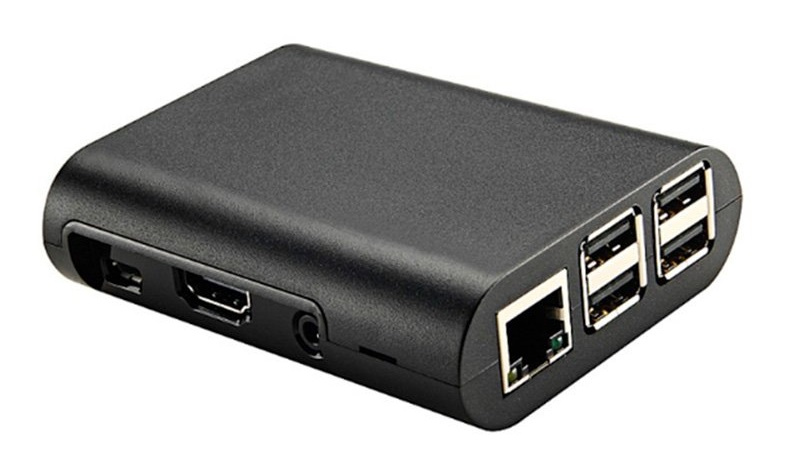
\includegraphics[height=9cm]{case_oval}
    \caption{Внешний вид корпуса Waveshare Electronics 11619}
    \label{pic:case_oval}
\end{figure}

\begin{figure}[h]
    \center
    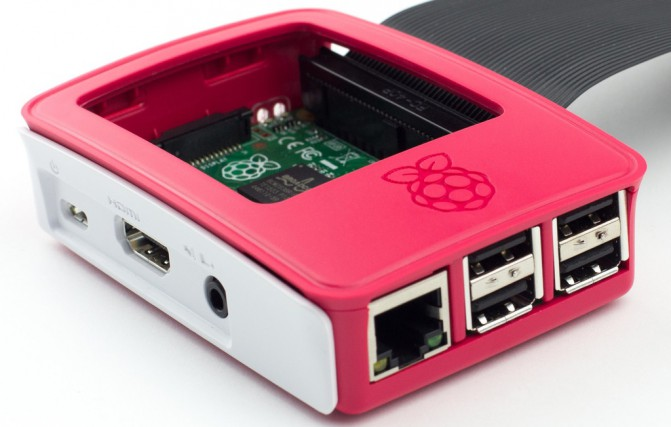
\includegraphics[height=9cm]{case_off}
    \caption{Внешний вид корпуса Waveshare Electronics 11655 с установленной платой
    Raspberry Pi}
    \label{pic:case_off}
\end{figure}

\begin{figure}[h]
    \center
    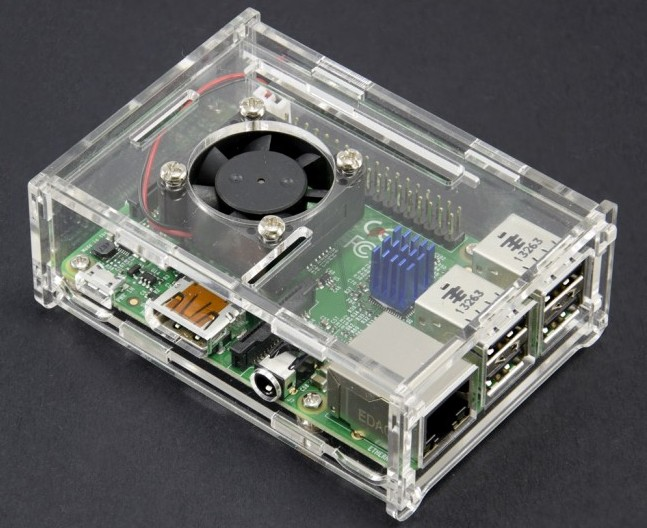
\includegraphics[height=9cm]{case_fan}
    \caption{Внешний вид корпуса Seeed Studio 114990129}
    \label{pic:case_fan}
\end{figure}

\clearpage
\section{Техническое задание}

Техническое задание на разработку тонкого клиента на базе микрокомпьютера, шифр «Клиент»

\begin{easylist}[articletoc]
\ListProperties(Progressive*=3ex,Hide4=4)
@ Цель выполнения ТЗ, наименование
@@ Целью выполнения ТЗ шифр «Клиент» является разработка тонкого клиента с корпусом,
изготовленным с помощью аддитивных технологий
@@ Наименование изделия: Тонкий клиент
@@ Краткое наименование изделия: изделие «Клиент»
@ Тактико-технические требования к изделию
@@ Состав изделия «Клиент»
@@@ Изделие «Клиент» должно включать одно или более твердых тел, объединенных в корпус
@@@ В состав корпуса предполагается установка платы микрокомпьютера Raspberry~Pi 3B c
microSD-картой
@@ Конструктивные требования
@@@ Масса изделия не должна превышать 300 г
@@@ Материалы, возможные для использования: 
@@@@ — Пластик на основе полилактида (PLA)
@@@@ — ABS-пластик
@@@@ — Пластик PET-G
@@ Требования назначения
@@@ В изделии должен быть доступ к разъемам микрокомпьютера Raspberry~Pi:
@@@@ — USB-A
@@@@ — HDMI
@@@@ — Ethernet (RJ-45)
@@@@ — Разъем питания microUSB
@@@ Должно быть предусмотрено отверстие для подключения и извлечения microSD-карты
@@@ Электропитание изделия «Клиент» должно осуществляться от сети
переменного тока напряжением 220 В ± 10\%, частотой 50 Гц ± 10\%.
@@ Требования живучести и стойкости к внешним воздействиям
@@@ Синусоидалльная вибрация, амплитуда ускорения 10 м/с², диапазон частот 1–35 Гц.
@@@ Механический удар многократного действия с пиковым ускорением 60 м/с², длительность
действия ударного ускорения 15 мс.
@@ Требования транспортабельности
@@@ Упаковка изделия «Клиент» должна допускать его транспортирование
в условиях группы Жт по ГОСТ В 9.001-72 при условии исключения воздействия
на упаковку атмосферных осадков. В транспортном средстве упаковка с
изделием «Корпус РЭА» должна быть закреплена.
@@@ Условия транспортирования изделия «Клиент» в части воздействия
климатических факторов должны соответствовать условиям его хранения в
неотапливаемых помещениях по ГОСТ В 9.003-80 при температуре от минус
40°С до 50°С.
\end{easylist}



\section{Установка и настройка комплекса}

\subsection{Подготовка серверной ОС}

Для установки используется бесплатная демо-версия, позволяющая использовать все функции
ОС в течение 180 дней. Для тестирования будет использована версия Standart, т.к.
версия Essentials активируется только после ввода лицензионного ключа. Процесс установки
показан на рисунках \ref{pic:install-1}–\ref{pic:install-4}.

\begin{figure}[h]
    \center
    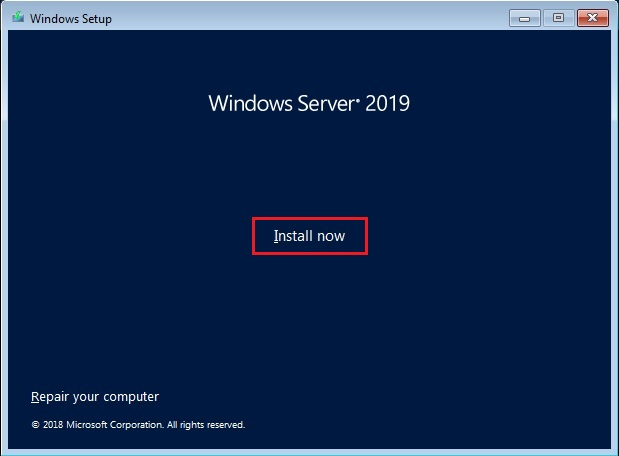
\includegraphics[height=8cm]{install-1}
    \caption{Главное окно установщика}
    \label{pic:install-1}
\end{figure}

\begin{figure}[p]
    \center
    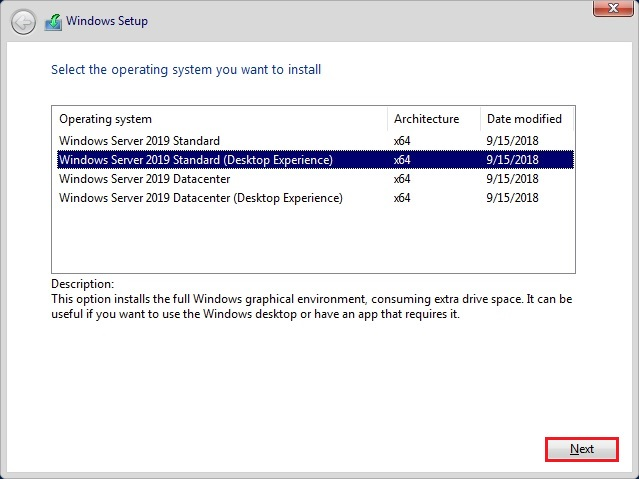
\includegraphics[height=10cm]{install-2}
    \caption{Выбор редакции}
    \label{pic:install-2}
\end{figure}

\begin{figure}[p]
    \center
    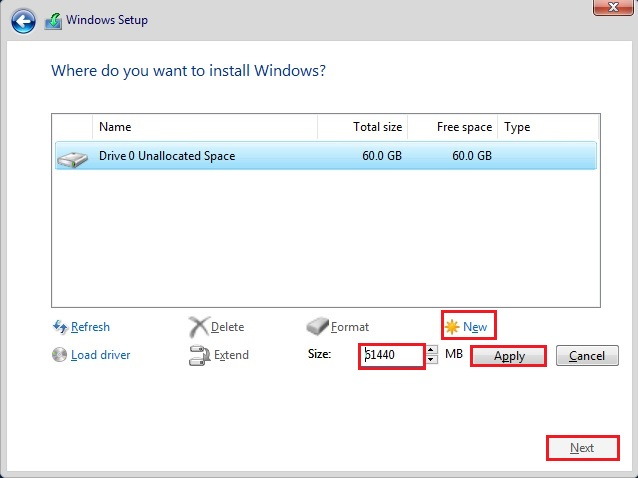
\includegraphics[height=10cm]{install-3}
    \caption{Выбор диска для установки}
    \label{pic:install-3}
\end{figure}

\begin{figure}[p]
    \center
    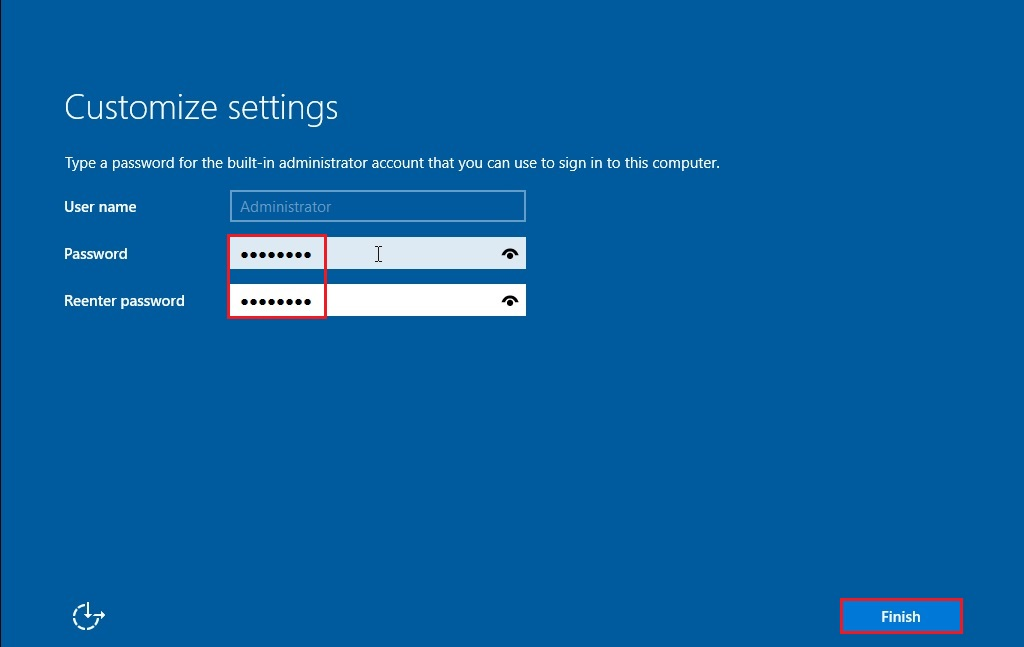
\includegraphics[height=10cm]{install-4}
    \caption{Создание учетной записи администратора}
    \label{pic:install-4}
\end{figure}

\begin{figure}[p]
    \center
    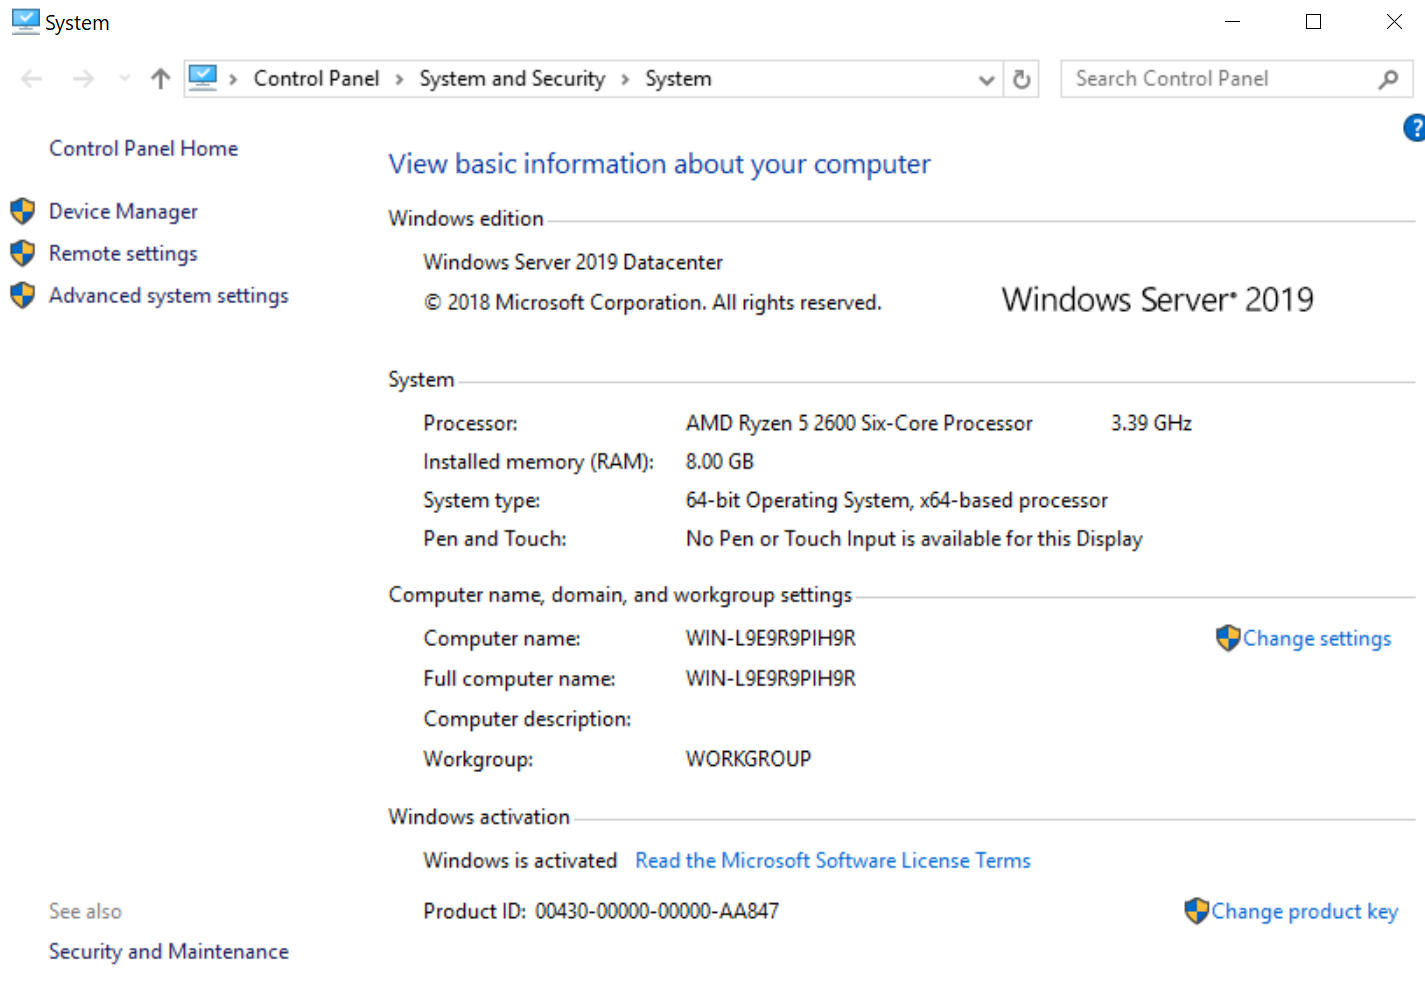
\includegraphics[height=10cm]{install-info}
    \caption{Сведения о установленной системе}
    \label{pic:install-info}
\end{figure}

\begin{figure}[p]
    \center
    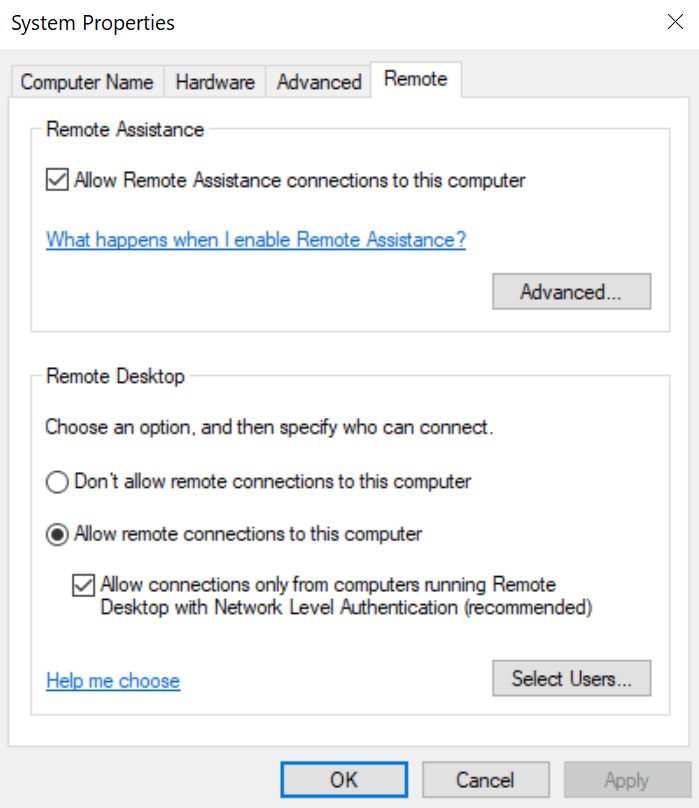
\includegraphics[height=10cm]{install-rdp}
    \caption{Включение доступа по RDP}
    \label{pic:install-rdp}
\end{figure}

\begin{figure}[h]
    \center
    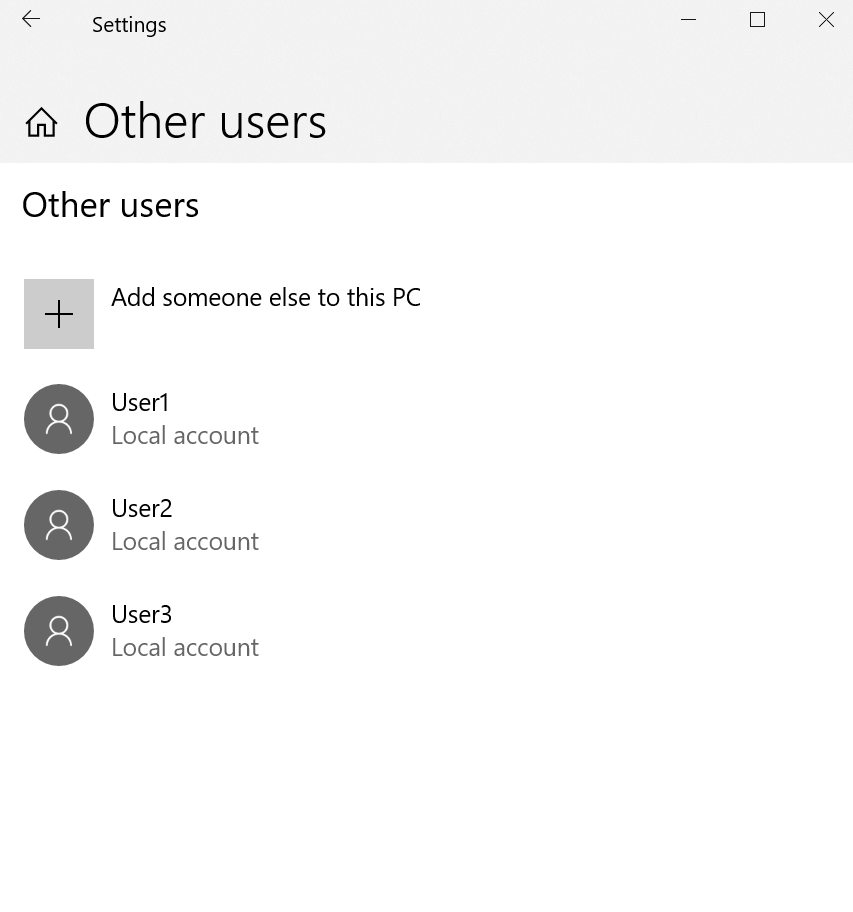
\includegraphics[height=10cm]{install-users}
    \caption{Добавление пользователей}
    \label{pic:install-users}
\end{figure}

В результате установки доступны все функции Windows Server (см.
рисунок~\ref{pic:install-info}). Нужно добавить возможность подключения по RDP
(см. рисунок~\ref{pic:install-rdp}). Также для работы нужно добавить в систему пользователей
для тонких клиентов. Добавлены пользователи \texttt{User1} – \texttt{User3} (см.
рисунок~\ref{pic:install-users}). Установка клиентского ПО (различные САПР, офисные
пакеты и т.д.) в работе не рассматривается.

\clearpage
\clearpage
\subsection{Подготовка клиентов}

Для того, чтобы подготовить к работе терминал, нужно установить ОС, RDP-клиент, и 
настроить автоматическое подключение к серверу.

С официального сайта \cite{ref:raspbian} необходимо скачать iso-образ Raspbian, версии
Lite без рабочего стола. Для установки ОС на microSD карту используется Etcher
\cite{ref:etcher}. Выбирается загруженный образ, нужный носитель и производится запись
(см. рисунок~\ref{pic:rpi-etcher}).

\begin{figure}[h]
    \center
    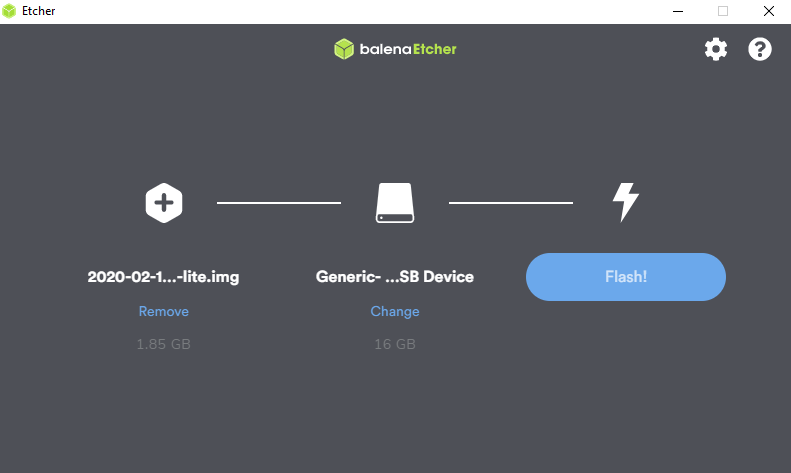
\includegraphics[width=\linewidth]{rpi-etcher}
    \caption{Запись iso на SD-карту с помощью Etcher}
    \label{pic:rpi-etcher}
\end{figure}

\begin{figure}[h]
    \center
    
\includegraphics[width=\linewidth]{rpi-etcher-complete}
    \caption{Подтверждение успешной записи}
    \label{pic:rpi-etcher-complete}
\end{figure}

\begin{figure}[h]
    \center
    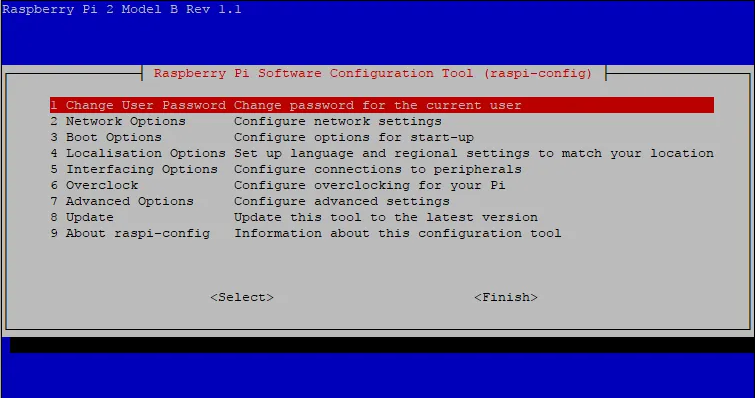
\includegraphics[width=\linewidth]{raspi-config}
    \caption{Окно утилиты \texttt{raspi-config}}
    \label{pic:raspi-config}
\end{figure}

После подтверждения успешной записи (см. рисунок~\ref{pic:rpi-etcher-complete}) можно
выходить из программы. Далее microSD–карта устанавливается в Raspberry Pi, подключаются
источник питания, сетевой кабель (на данном этапе нужен доступ в Интернет), клавиатура 
и монитор. После загрузки необходимо авторизоваться (по умолчанию логин — 
\texttt{pi}, пароль — \texttt{raspberry}). Теперь доступен режим работы с командной
строкой.

Нужно установить раскладку клавиатуры \texttt{en\_US.UTF-8} и выбрать часовой пояс. Это
можно сделать с помощью программы \texttt{raspi-config} (см.
рисунок~\ref{pic:raspi-config}) в пункте Localisation Options.  Также необходимо сменить
пароль для пользователя \texttt{pi} (Change User Password), а также выбрать режим
автоматического входа в систему (Boot Options — Desktop/CLI — Console autologin).

Обновление каталога ПО и установка нужных пакетов выполняется следующими командами:
\begin{verbatim}
sudo apt update && sudo apt upgrade
sudo apt install --no-install-recommends xserver-xorg \
    x11-xserver-utils xinit openbox
sudo apt install freerdp2-x11 pulseaudio
\end{verbatim}

Теперь нужно настроить действия при загрузке сеанса. Редактируется файл
\texttt{/etc/xdg/openbox/autostart}, в котором будет вызываться RDP-клиент:
\begin{verbatim}
# Отключить все функции энергосбережения
xset s off
xset s noblank
xset -dpms

# Завершение сеанса по Ctrl-Alt-Backspace
setxkbmap -option terminate:ctrl_alt_bksp

# Запуск RDP с нужными параметрами
while true; do
  xfreerdp /fonts /bpp:15 /f /audio-mode:0 /u:[user] /p:[password] \
    /v:[ip] /gdi:hw /sound:sys:pulse /gfx:rfx /rfx-mode:video \
    +bitmap-cache +offscreen-cache -clipboard
done
\end{verbatim}

Нужно заменить поля в квадратных скобках на пользователя, пароль и IP-адрес сервера.
Теперь можно проверить работоспособность системы, загрузившись в графический режим:
\begin{verbatim}
startx --
\end{verbatim}

\begin{figure}[p]
    \center
    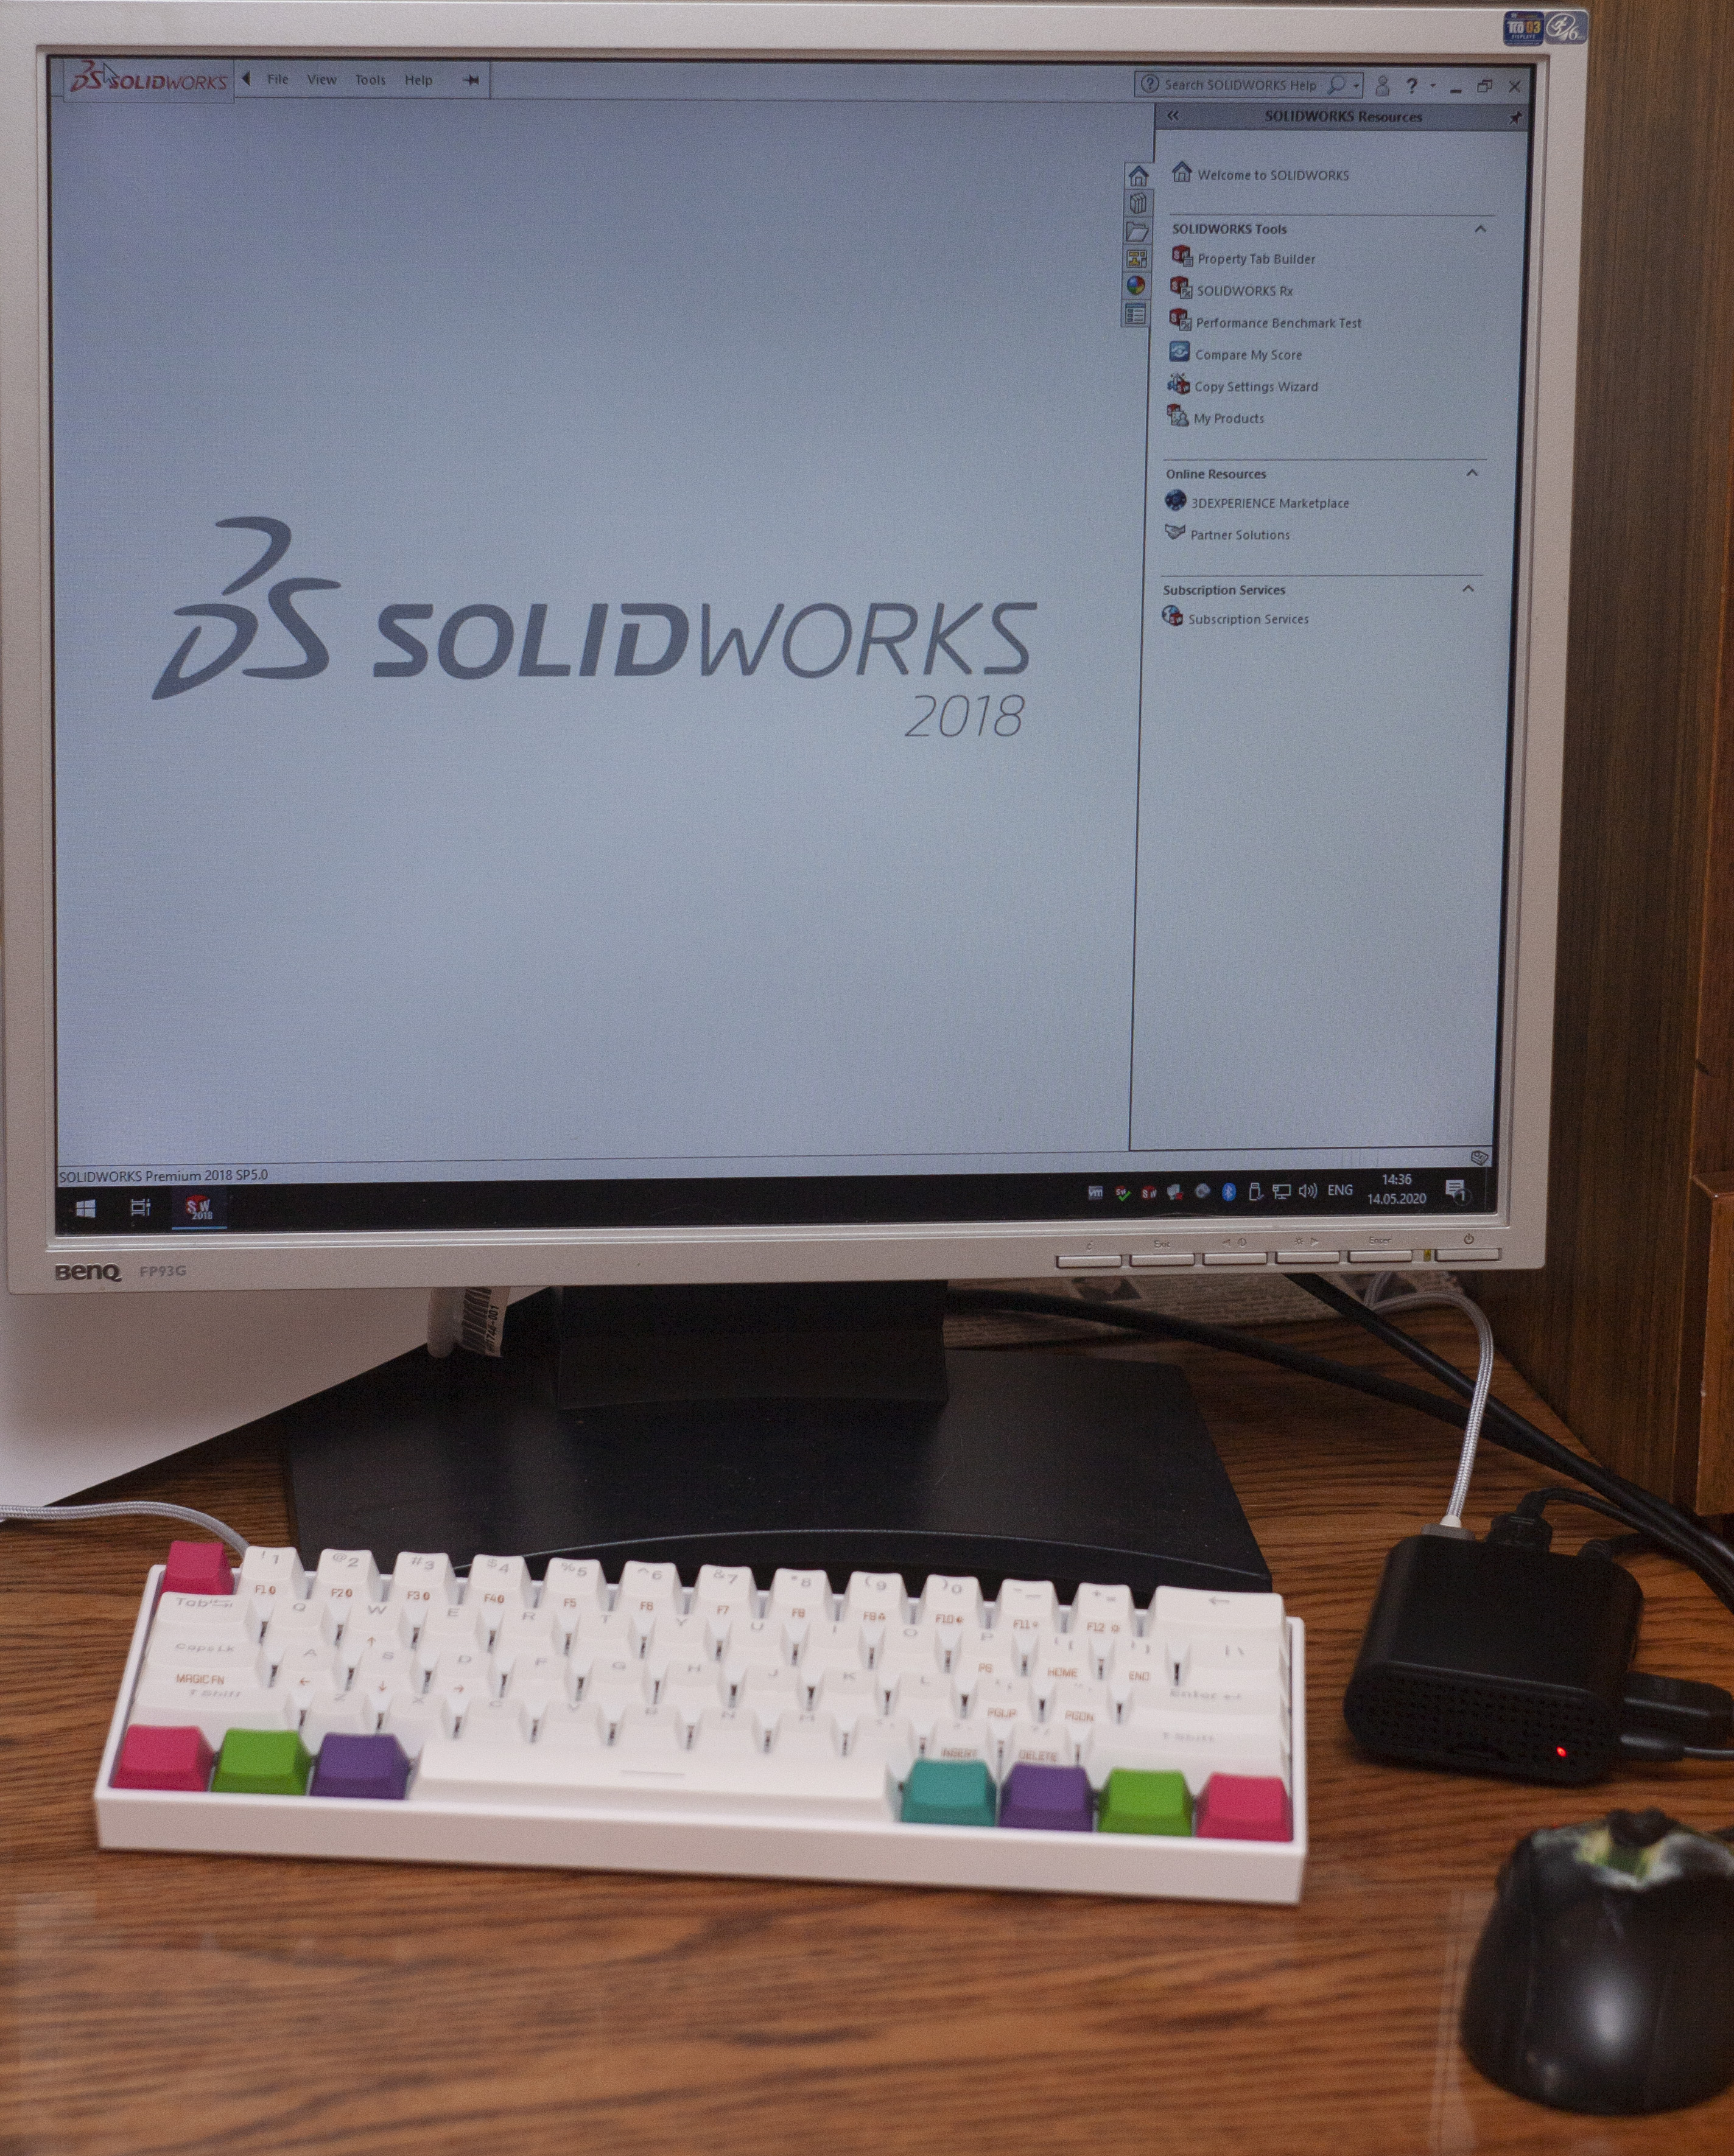
\includegraphics[width=\linewidth]{ph-solid}
    \caption{Готовый к работе тонкий клиент}
    \label{pic:ph-solid}
\end{figure}

Запускается RDP-клиент. Подключение к удаленному рабочему столу успешно (см.
рисунок~\ref{pic:ph-solid}). Завершается сеанс нажатием комбинации клавиш
Ctrl-Alt-Backspace. Осталось только прописать автоматическую загрузку сеанса. Для этого
в конец файла \texttt{~/.bash\_profile} нужно добавить следующую строку:
\begin{verbatim}
[[ -z $DISPLAY && $XDG_VTNR -eq 1 ]] && startx --
\end{verbatim}

После этого можно перезагрузить систему. После загрузки автоматически установится
RDP-соединение. Комбинация клавиш Ctrl-Alt-Backspace закрывает сеанс и возвращает в
консоль, это можно использовать при необходимости поменять конфигурацию. В графический
режим можно вернуться командой \texttt{startx --}, а комбинация клавиш Ctrl-D
перезапустит сеанс и так же загрузит графический режим.

Теперь с помощью программы Win32 Disk Imager \cite{ref:win32di} можно создать образ уже
настроенной системы, чтобы не настраивать каждый клиент отдельно. Далее можно будет на
карту памяти каждого клиента записать этот образ, после чего клиент будет готов к
работе. Останется только изменить логин и пароль пользователя в файле
\texttt{/etc/xdg/openbox/autostart}. Для создания такого образа нужно извечь карту
памяти из микрокомпьютера, вставить ее в ПК и открыть программу Win32 Disk Imager. В
окне нужно выбрать файл, в который будет записан образ системы, проверить соответствие
устройства и нажать кнопку Read (см. рисунок~\ref{pic:win32di}). Для уменьшения размера
образа можно воспользоваться опцией Read Only Allocated Partitions. Через некоторое
время образ будет считан. Теперь можно записывать его с помощью программ Etcher (так же,
как в начале установки) или Win32 Disk Imager (кнопка Write, затем Verify Only для
подтверждения корректности записи).

\begin{figure}[p]
    \center
    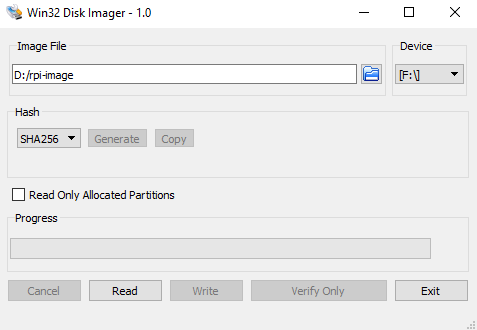
\includegraphics[width=\linewidth]{win32diskimager}
    \caption{Окно Win32 Disk Imager}
    \label{pic:win32di}
\end{figure}

В дальнейшем при модернизации системы можно настроить TFTP-сервер, который позволит
загружать тонкие клиенты по сети, что позволит избавиться от неободимости в карте
памяти для каждого устройства и еще больше упростит конфигурацию новых клиентов. Однако
это увеличит время загрузки каждого клиента, т.к. придется скачивать весь образ по сети
при каждой загрузке.

\section{Корпус изделия}
В соответствии с техническим заданием был разработан корпус для тонкого клиента.
Трехмерная модель корпуса представлена на рисунке (см. рисунок~\ref{pic:case}), сборка
изделия — на рисунке (см. рисунок~\ref{pic:assy}).

Фотографии изделия в сборе представлены на
рисунках~\ref{pic:assy_photo_1},~\ref{pic:assy_photo_2}.

\begin{figure}[h]
    \center
    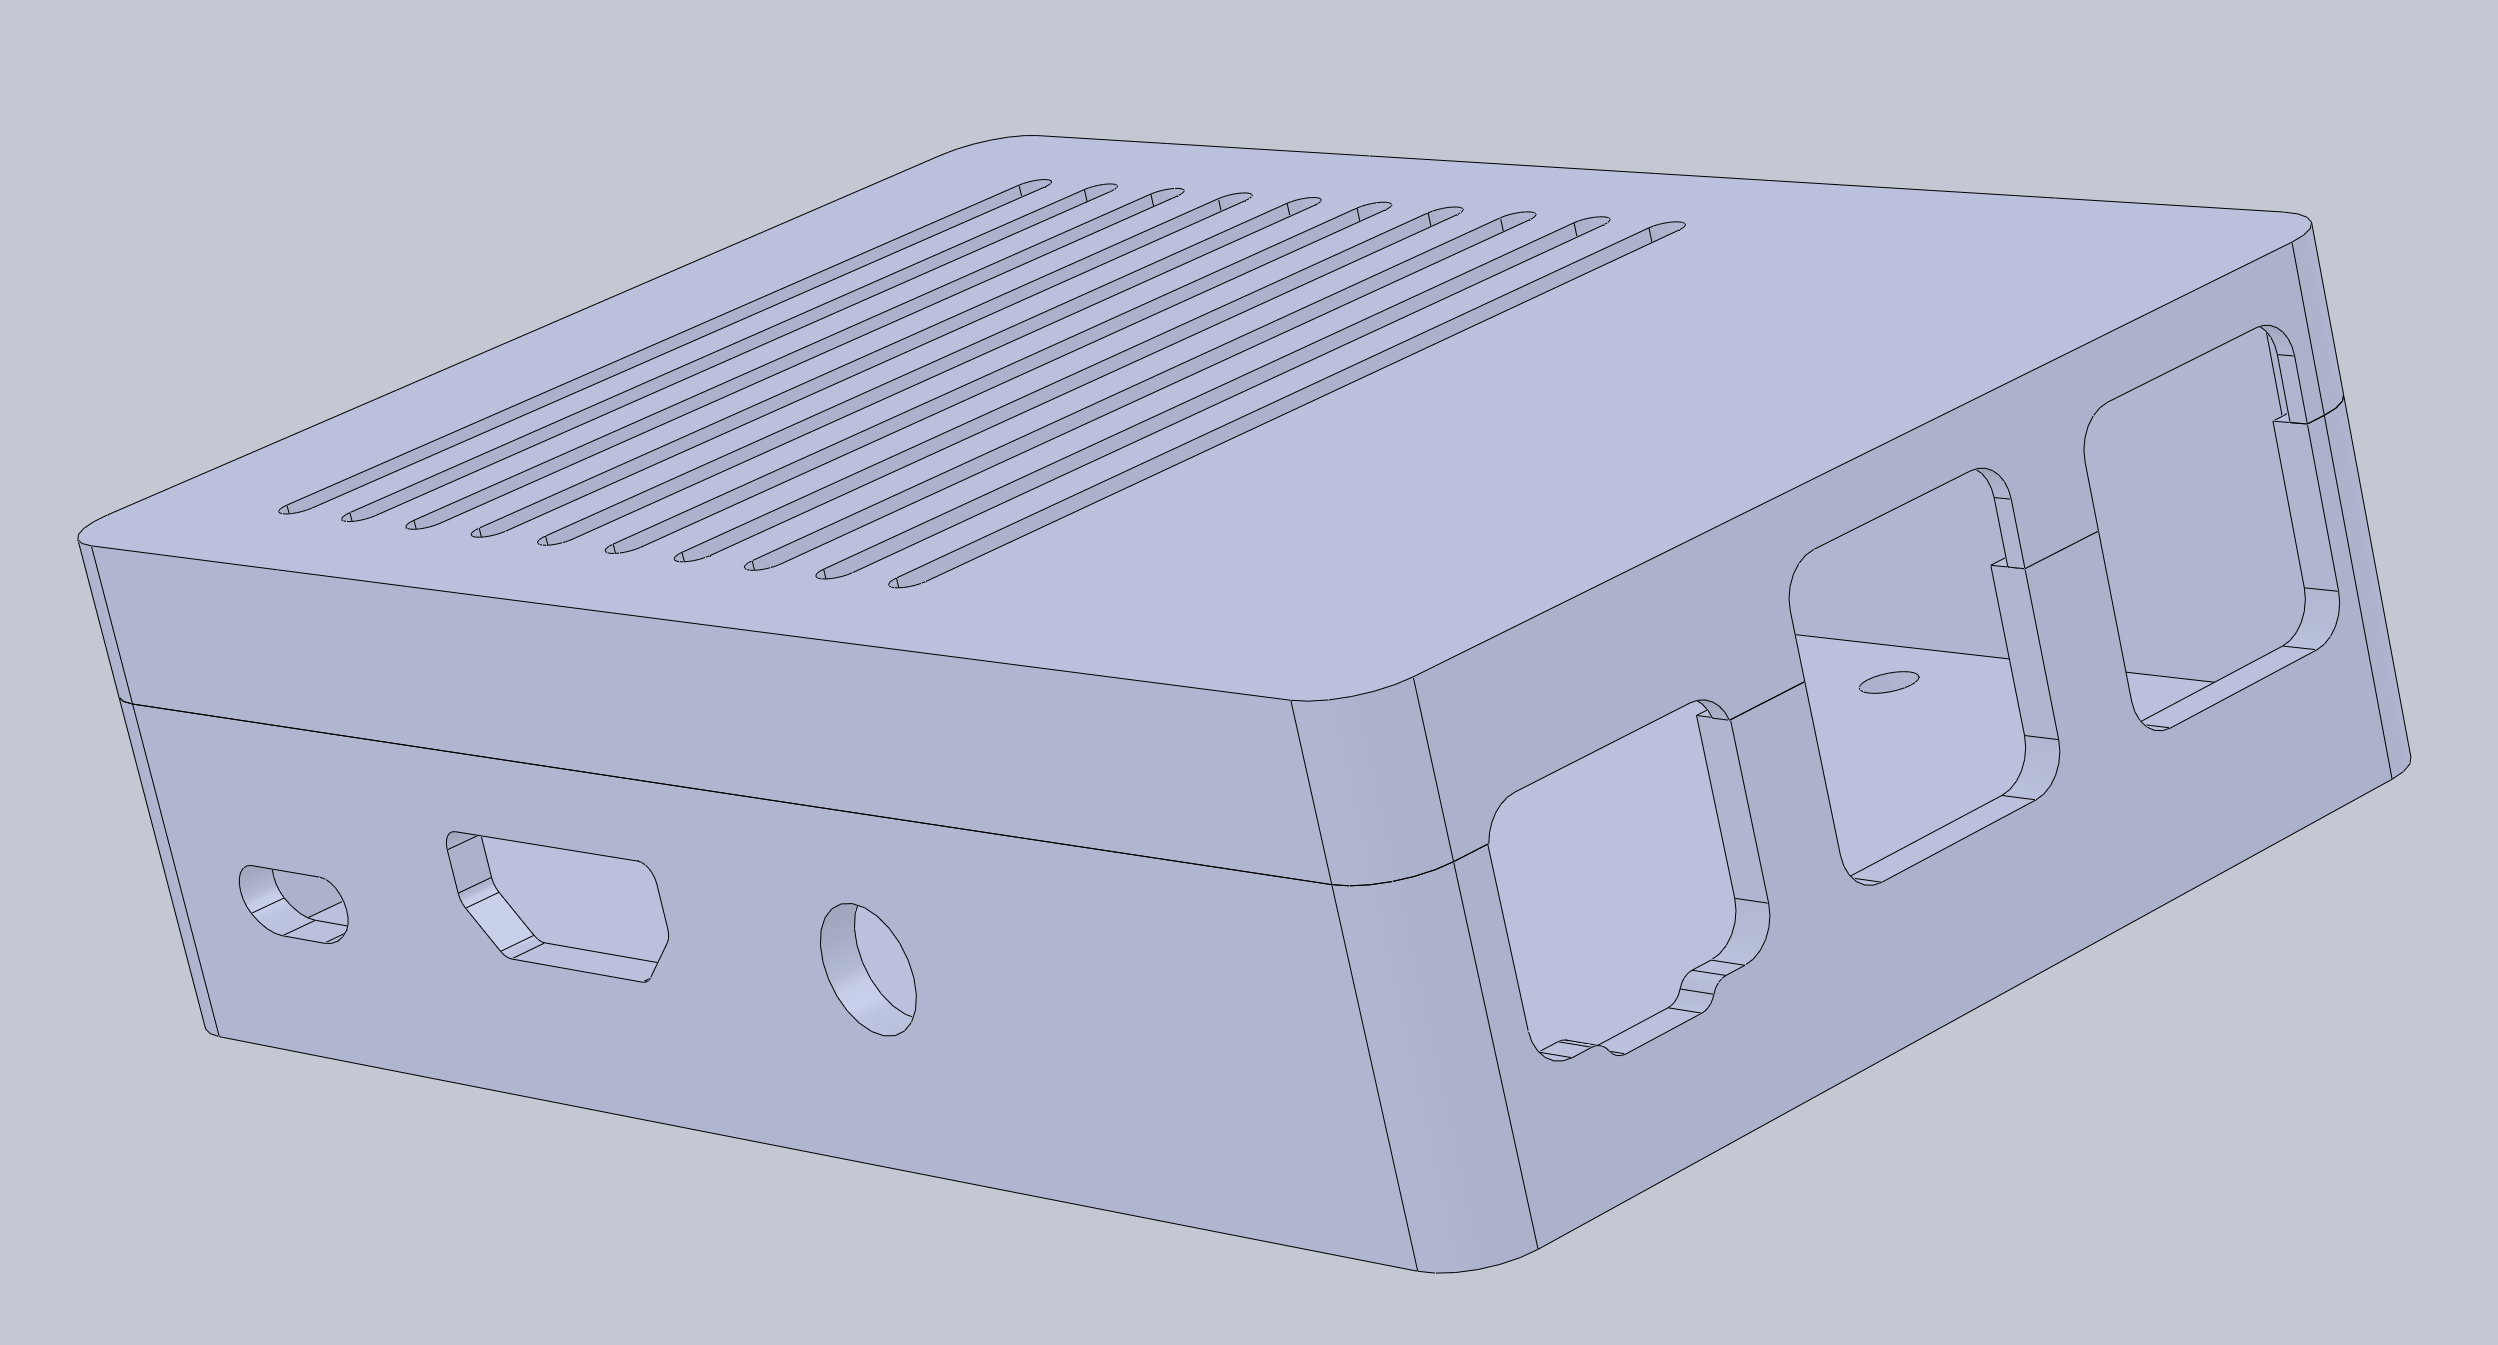
\includegraphics[height=6cm]{case}
    \caption{Модель корпуса}
    \label{pic:case}
\end{figure}

\begin{figure}[h]
    \center
    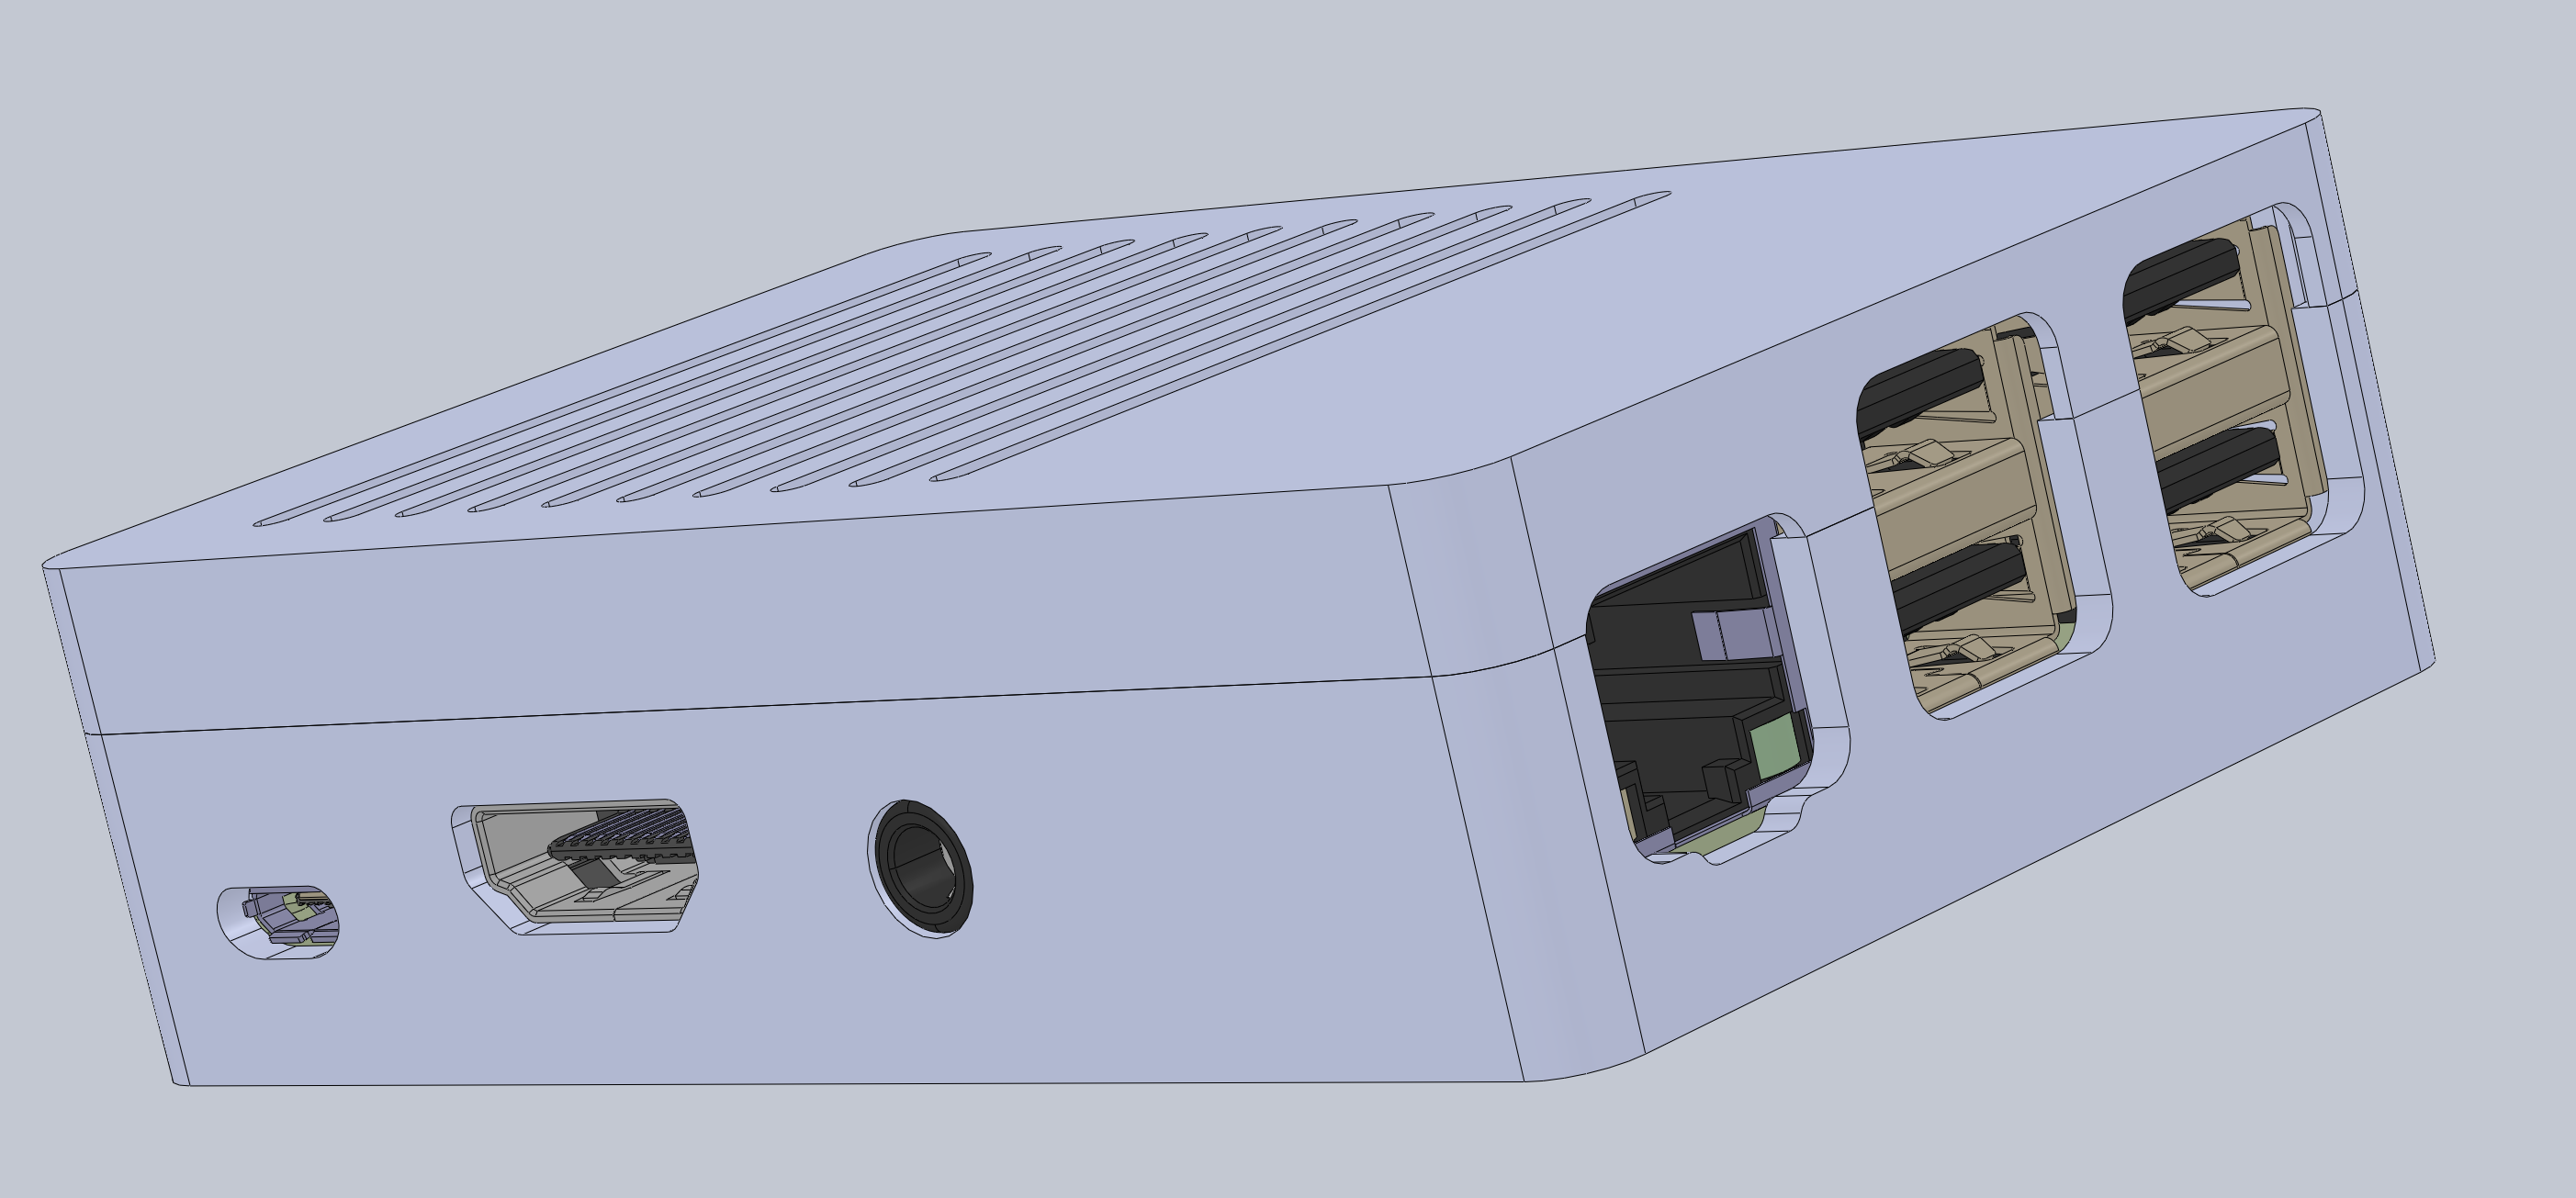
\includegraphics[height=8cm]{assy}
    \caption{Модель сборки}
    \label{pic:assy}
\end{figure}

\begin{figure}[h]
    \center
    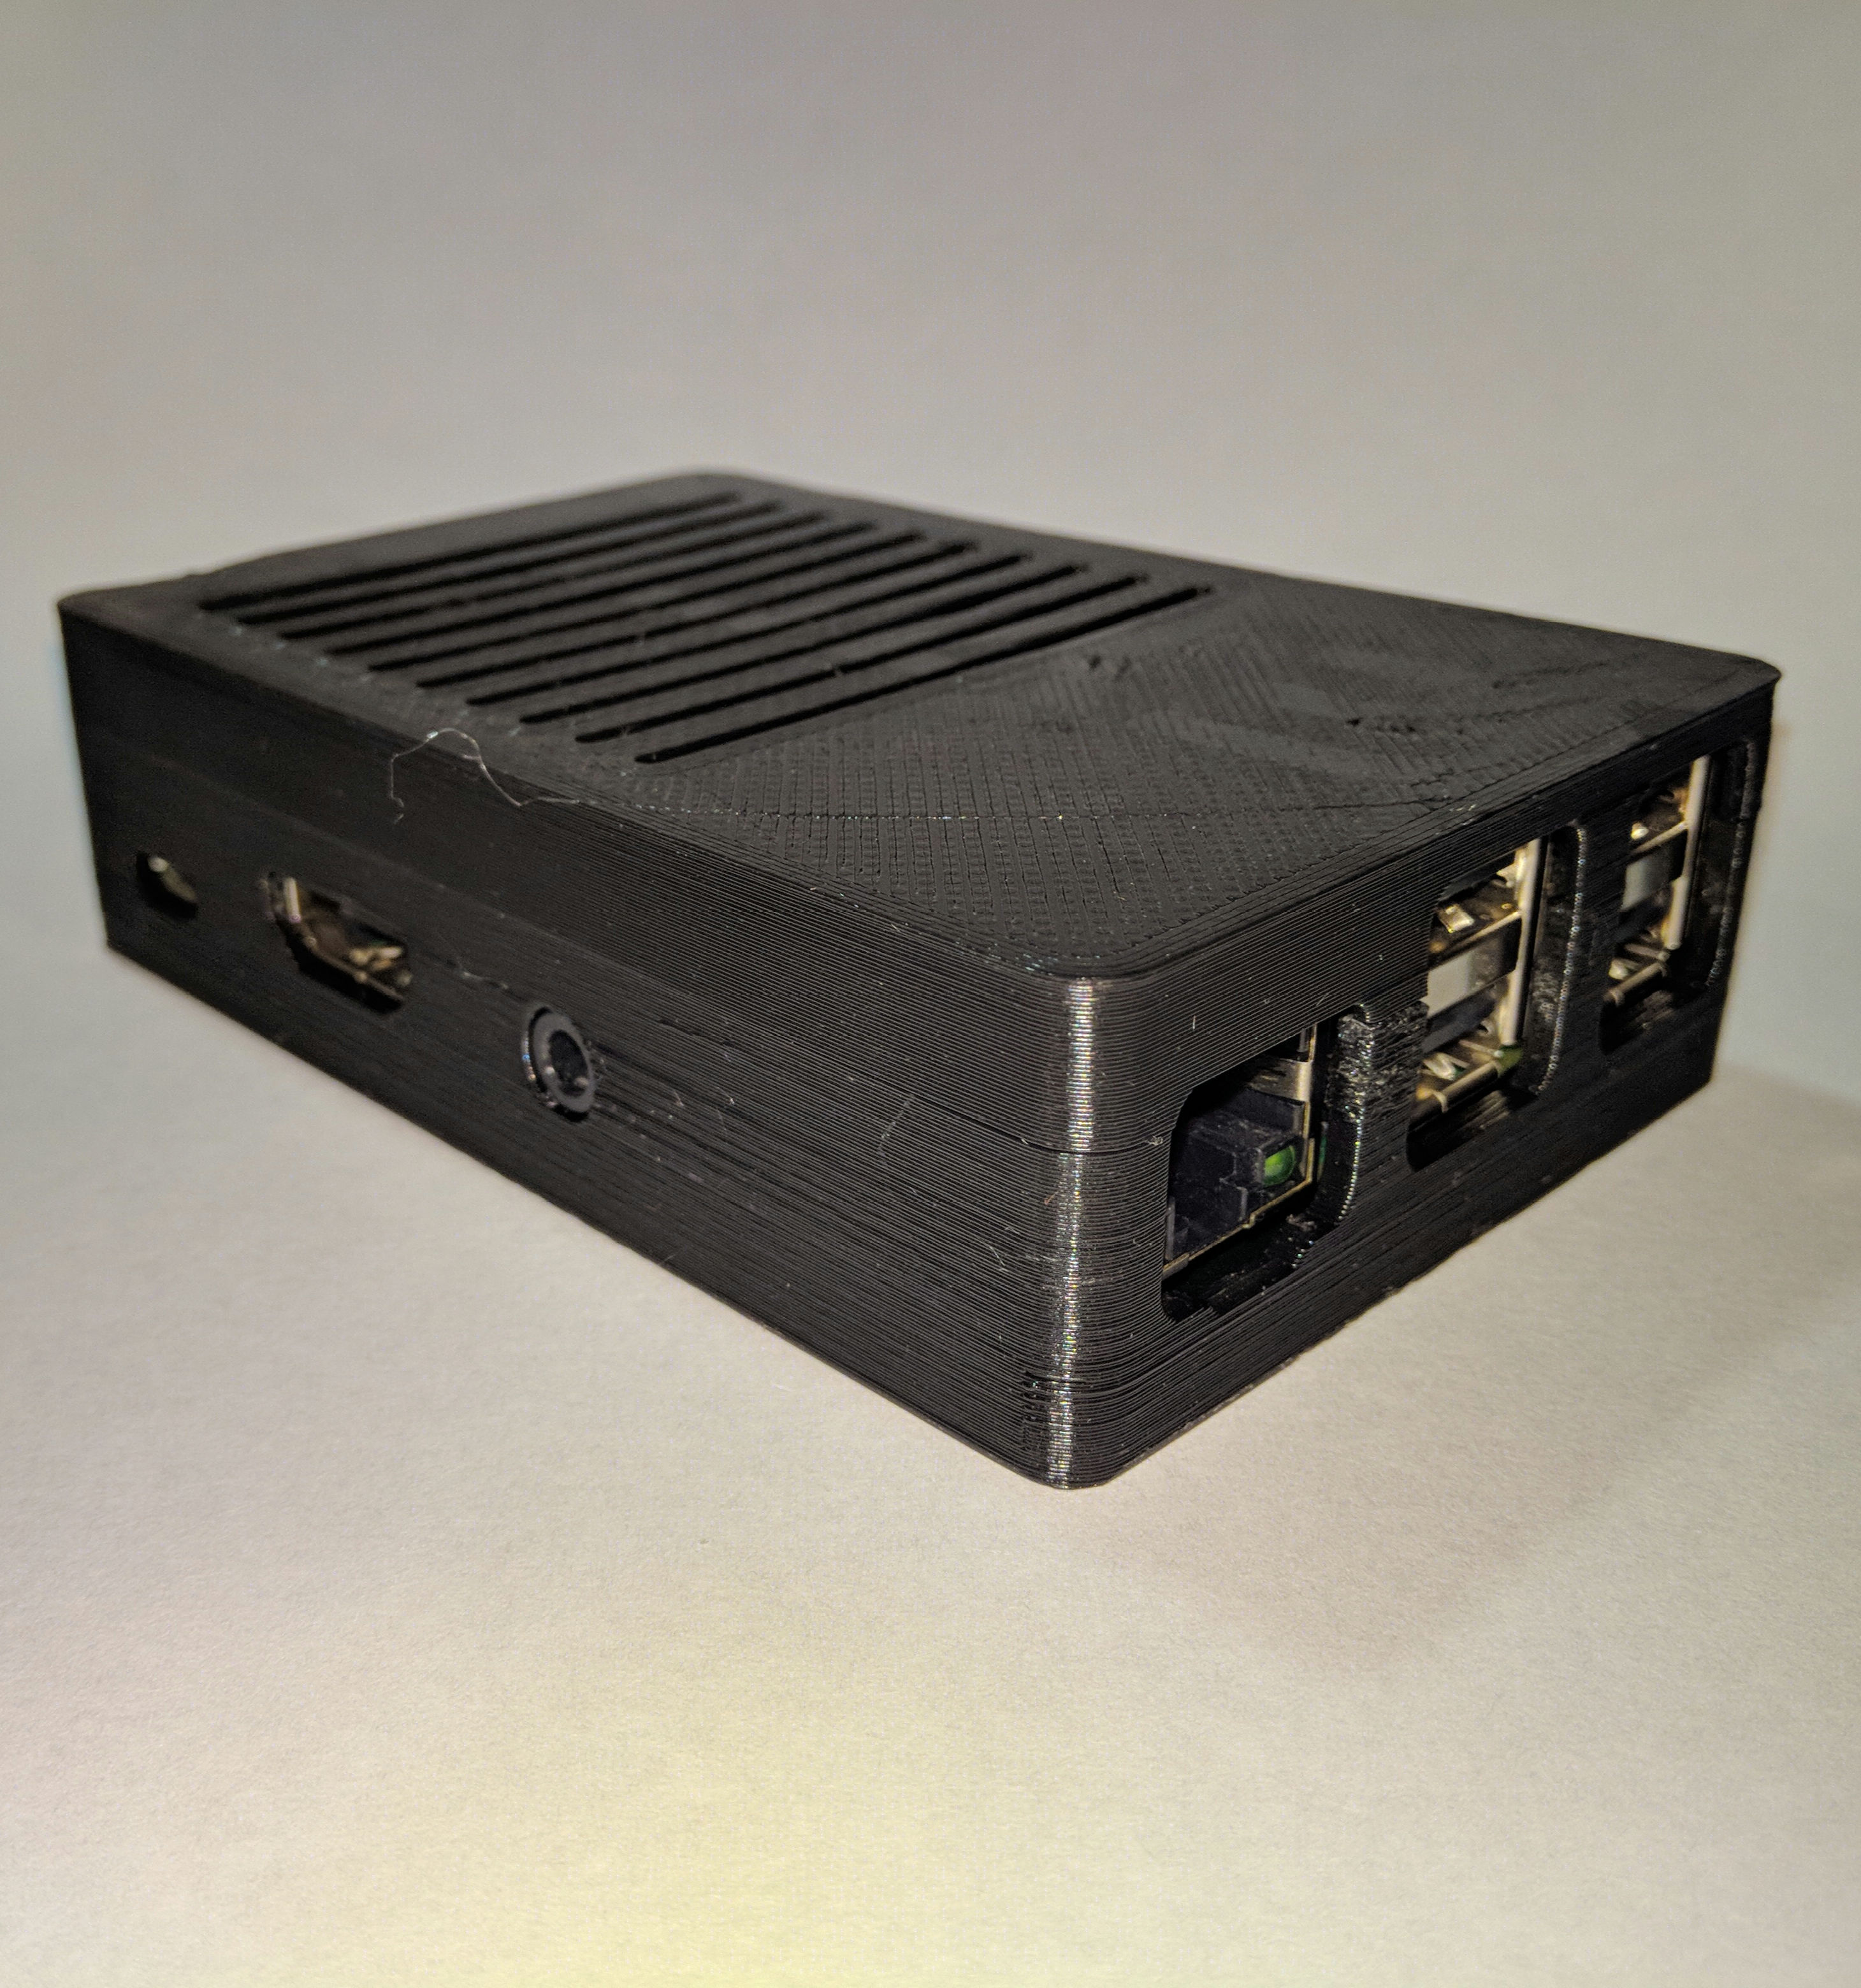
\includegraphics[height=10cm]{assy_photo_1}
    \caption{Устройство в сборе}
    \label{pic:assy_photo_1}
\end{figure}

\begin{figure}[h]
    \center
    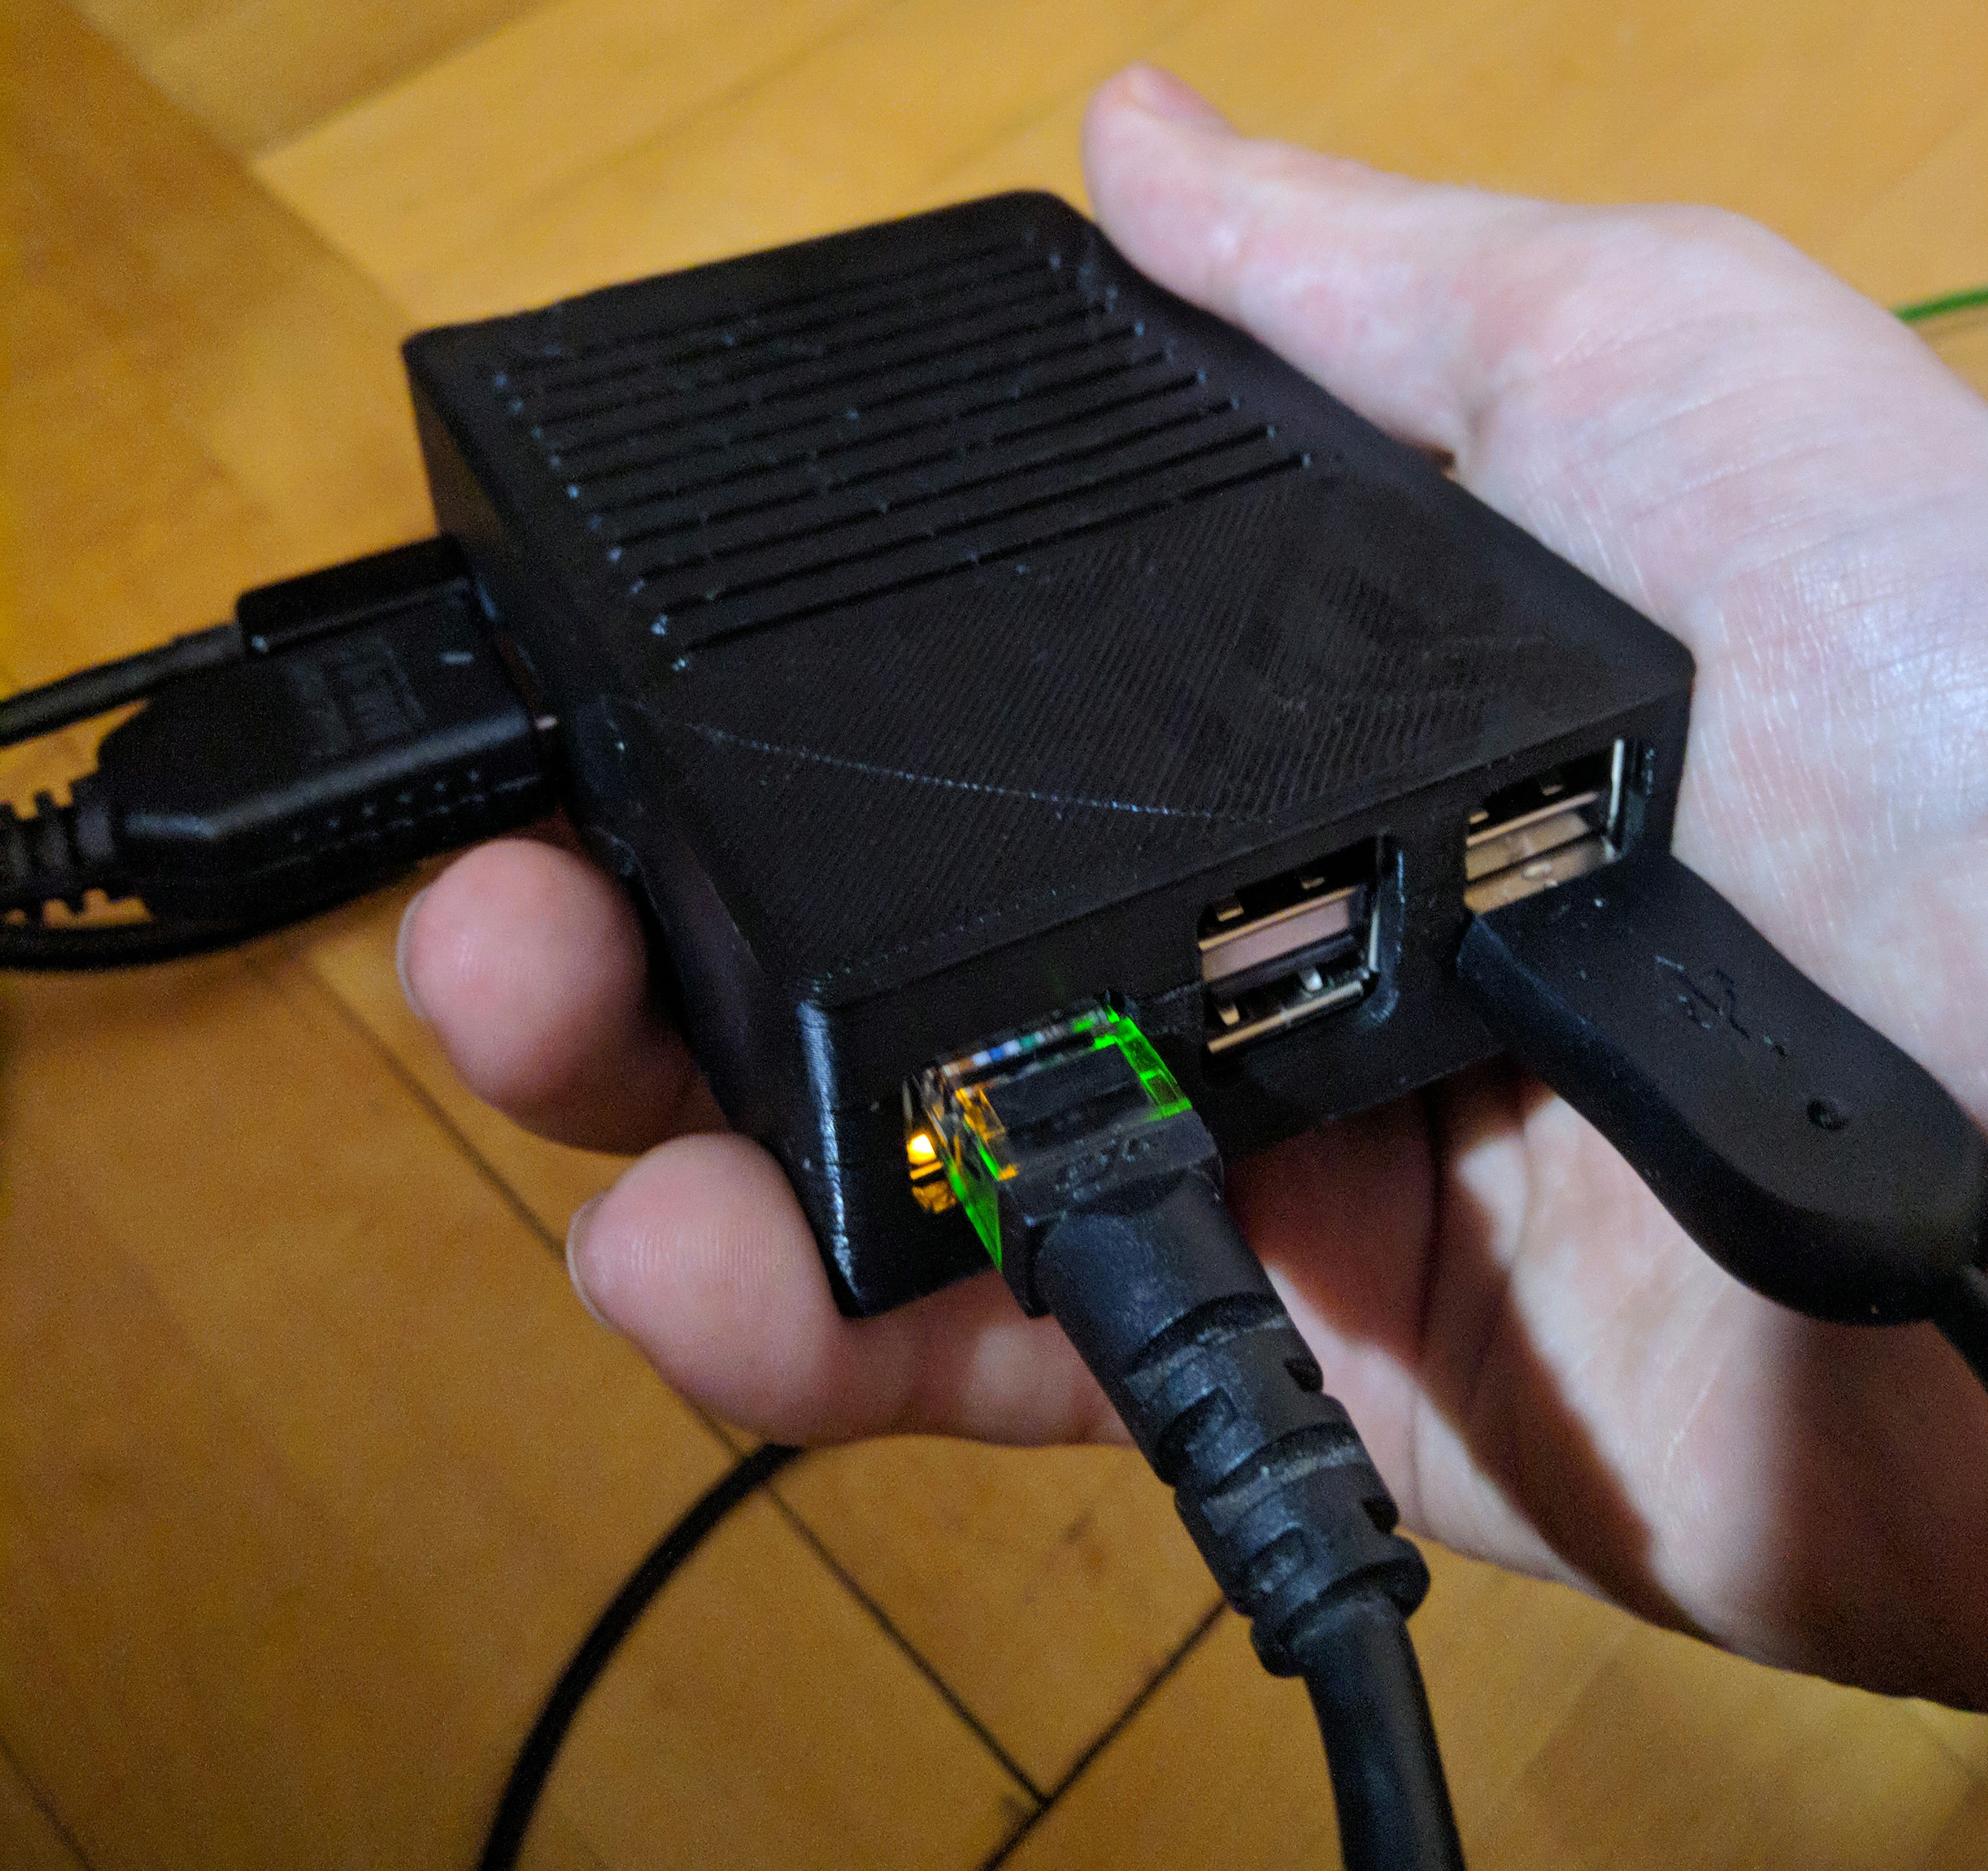
\includegraphics[width=\linewidth]{assy_photo_2}
    \caption{Устройство в работе}
    \label{pic:assy_photo_2}
\end{figure}


\chapter{Анализ результатов работы}
\section{Тестирование производительности}

Производительность будет тестироваться с помощью встроенного в SolidWorks средства
SOLIDWORKS Performance Test. В этом тесте проверяется производительность системы в
типичных для SolidWorks задачах. Тестирование будет производиться на следующих
конфигурациях аппаратного обеспечения:
\begin{enumerate}
    \item Компьютеры, используемые на кафедре КПРС. Тест производится для оценки
        изначальной производительности системы.
    \item Используемый сервер. Включен в тест для оценки чистой производительности
        сервера, а также для оценки падения производительности на клиентских машинах.
    \item Разработанные тонкие клиенты. Тест проводится на тонком клиенте и сервере
        одновременно для исследования влияния клиентов друг на друга. Тест отражает
        сценарий использования системы под нагрузкой.
    \item Тонкий клиент, тест запущен только на одном устройстве для верификации данных.
        Результаты должны быть идентичны пункту 2 (в пределах погрешности).
        Необходимо сравнить результаты с используемыми сейчас компьютерами для оценки
        изменения производительности всей системы.
\end{enumerate}

\begin{figure}[h]
    \center
    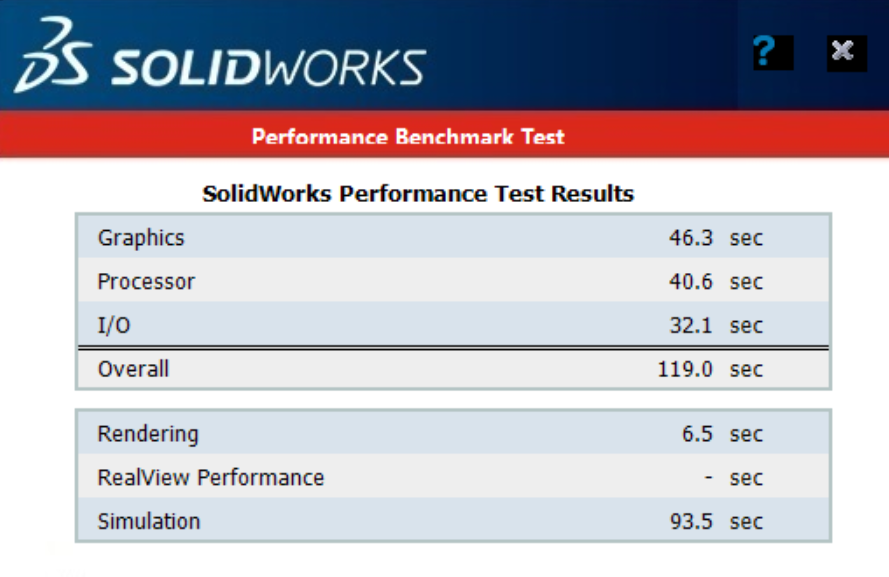
\includegraphics[width=\linewidth]{server_perf}
    \caption{Пример результата Solidworks Performance Test (2~конфигурация)}
    \label{pic:server_perf}
\end{figure}

Все тесты выполнялись 3 раза, результаты усреднены и представлены в сравнительной
таблице~\ref{tab:solid_comp}, а так же, для наглядности, на диаграмме (см.
рисунок~\ref{pic:perf_chart}). Данные показывают время выполнения одного теста и
представлены в секундах, меньше — лучше.

\begin{table}[h]
    \centering
    \caption{SOLIDWORKS Performance Test, средние значения}
    \label{tab:solid_comp}
    \begin{tabu}to \linewidth{XX[1,c,m]X[1,c,m]X[1,c,m]X[1,c,m]}
        \toprule
        Конфигурация & 1     & 2    & 3    & 4    \\
        \midrule
        Графика & 52,1 & 20,2 & 25,0 & 20,7 \\ 
Процессор & 51,0 & 30,5 & 30,2 & 29,4 \\ 
Ввод-вывод & 31,7 & 22,9 & 43,6 & 21,4 \\ 
Рендеринг & 7,6 & 5,6 & 6,8 & 5,6 \\ 
Симуляция & 105,0 & 44,6 & 55,7 & 43,2 \\ 

        \bottomrule
    \end{tabu}
\end{table}

\begin{figure}[h]
    \center
    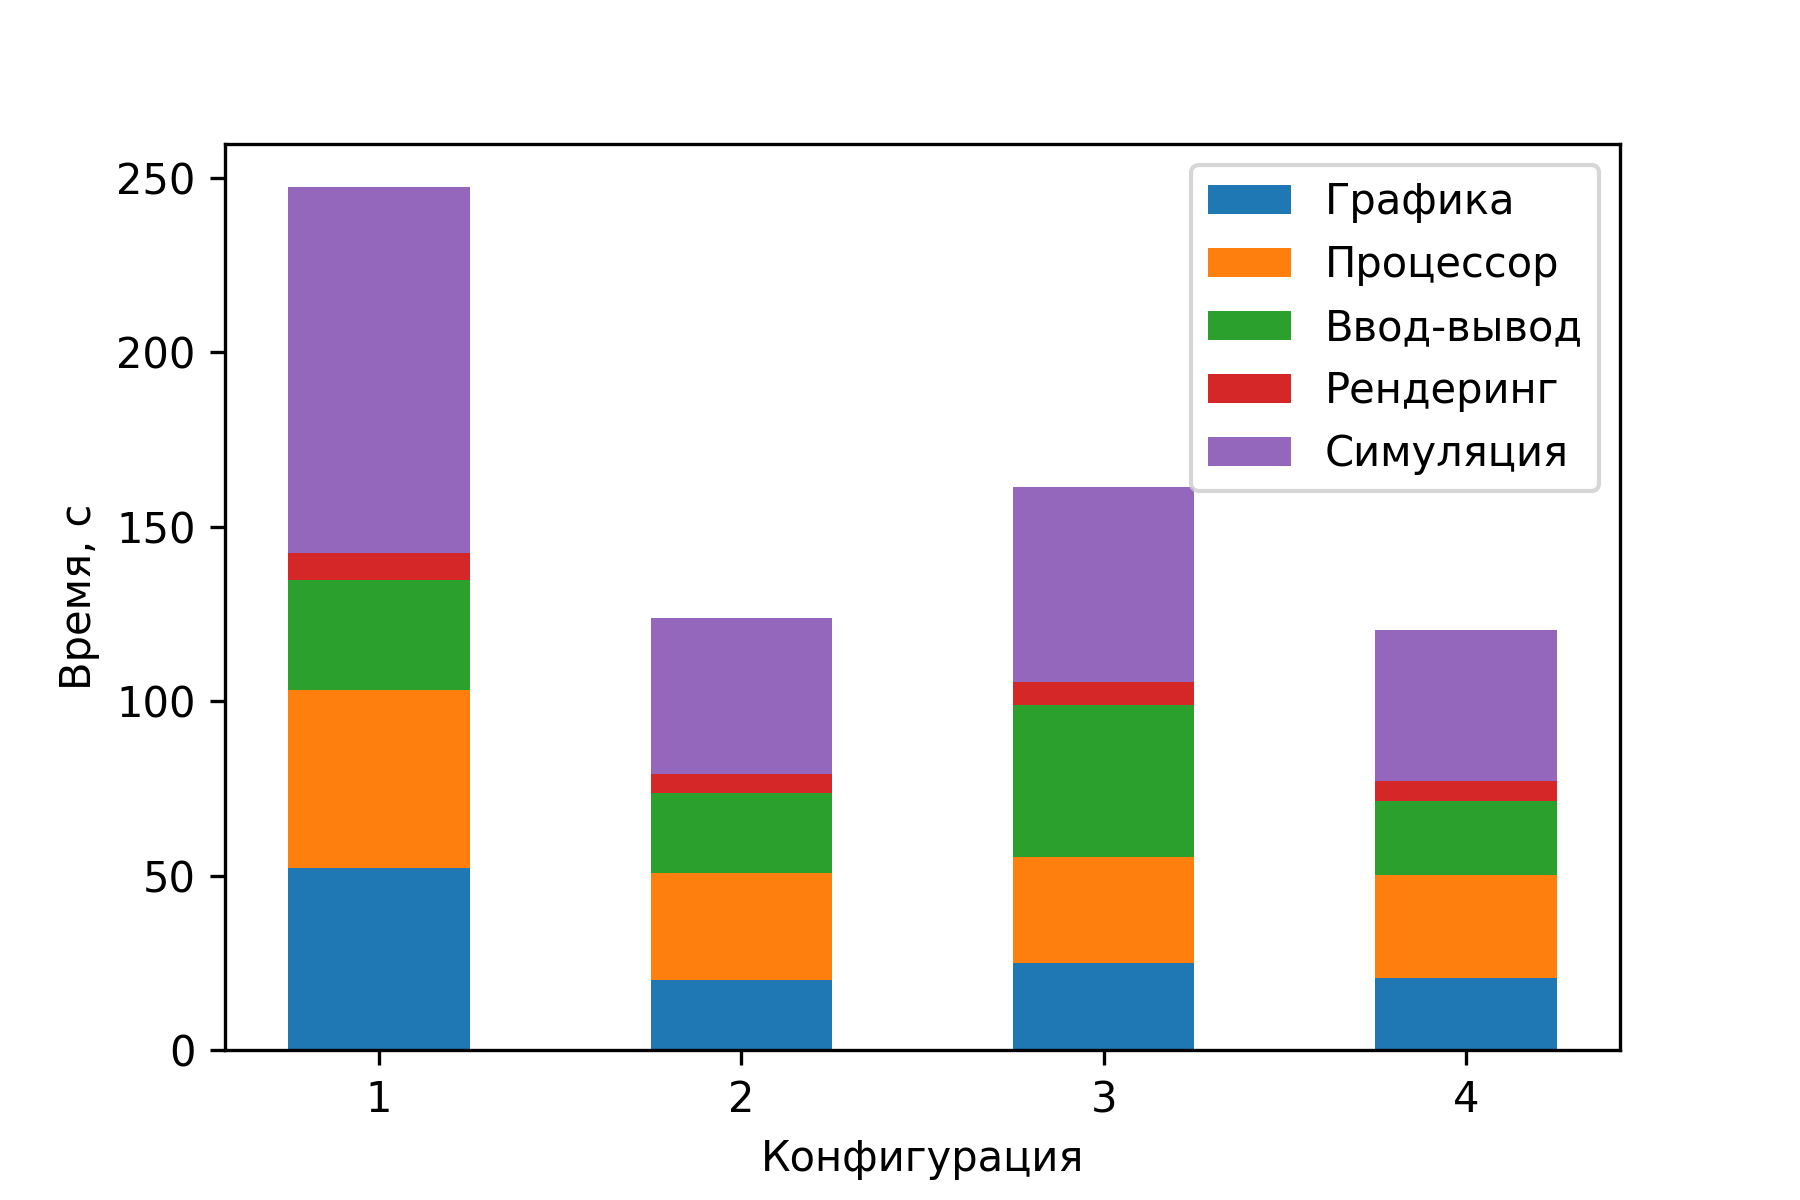
\includegraphics[width=\linewidth]{perf_chart}
    \caption{Результаты SOLIDWORKS Performance Test}
    \label{pic:perf_chart}
\end{figure}

В целом тест показывает прирост производительности при переходе на систему тонких
клиентов. Однако, в ходе тестирования были обнаружены следующие проблемы:
\begin{itemize}
    \item На некоторых компьютерах тест не запускался, зависал во время выполнения или
        не выдавал результатов. 
    \item Разброс значений даже в пределах одного устройства достаточно высок, что не
        дает возможности сделать вывод на основании этого теста. 
\end{itemize}

Для подтверждения результатов общевычислительной производительности, будет произведено
дополнительное тестирование в программе PCMark 10, редакция Basic Edition
\cite{ref:pcmark}. 
Программы серии PCMark тестируют стабильность и производительность работы процессоров,
скоростные характеристики и пропускную способность оперативной и постоянной памяти, а
также множество других характеристик компьютерных компонентов. Для тестирования
используются различные тесты, как синтетические, нагружающие определённые блоки
компьютера, так и прикладные, например архивация данных, кодирование и декодирование
аудио и видео, производительность физического движка и т. д. 
PCMark является стандартом в индустрии компютерного аппаратного обеспечения.

Конфигурации тестируемого оборудования остались прежними (кроме теста 3, т.к.
одновременный запуск разных тестов не имеет смысла), результаты тестирования
приведены в таблице~\ref{tab:pcmark_comp}. Результат для каждого теста выдается в виде
условных единиц, затем результаты всех тестов усредняются. Больше — лучше.

\begin{table}[h]
    \centering
    \caption{PCMark 10}
    \label{tab:pcmark_comp}
    \begin{tabu}to \linewidth{X[1,c,m]X[1,c,m]X[1,c,m]X[1,c,m]X[1,c,m]}
        \toprule
        Конфигурация & 1     & 2    & 3 & 4    \\
        \midrule
        Результат PCMark 10 & 2089 & 5276 & — & 5201 \\
        \midrule
        Итог &  &  &  &  \\
        \bottomrule
    \end{tabu}
\end{table}

Таким образом, по результатам проведенных тестов, можно сделать вывод о увеличении
производительности при использовании предложенной системы, состоящей из
производительного сервера и тонких клиентов в сценарии многопользовательской работы, по
сравнению с используемыми сейчас на кафедре компьютерами (толстыми клиентами). 

\section{Экономическая эффективность}

Для оценки экономической эффективности нужно сравнить затраты на аппаратное и
программное обеспечение, используемое в проекте. Цены на компьютерные комплектующие
взяты с сервиса агрегации цен E-katalog \cite{ref:eeekatalog}. Цены на ПО взяты с сайтов
официальных дистрибуторов ПО (или их представителей в Российской Федерации).  Для
отсутствующих в продаже компонентов взяты их современные аналоги, сравнимые по
производительности.

Так как сервер для демонстрации возможностей данного проекта собран из обычных
потребительских комплектующих, в таблице указана их стоимость. Стоит отметить, что для
сборки полноценного сервера стоит использовать специализированные серверные 
комплектующие. Их стоимость выше, однако и производительность при этом отличается в
большую сторону, что может быть полезно для дальнейшего увеличения производительности и
надежности всей системы.

Стоимость комплектующих сервера приведена в таблице \ref{tab:server_price},
комплектующих ПК — в таблице \ref{tab:pc_price}. В расчетах не учитывается стоимость
корпуса. Cтоимость Raspberry Pi 3 Model B, корпуса и блока питания в сумме принята
6000~рублей при покупке от 5~шт. \cite{ref:raspberry_price}. В расчетах не учитывается
стоимость мониторов, клавиатур и компьютерных мышек, так как они идентичны в обоих
сценариях.

Помимо аппаратного обеспечения, нужно учесть затраты на программное обеспечение для всех
клиентов. Т.к. Windows Server Essentials не требует дополнительных клиентских лицензий,
то стоимость лицензирования будет равна 17 158 руб. (для оценки взята стоимость
Microsoft Windows Server Essentials 2019, коробочная версия для академических
организаций). Для клиентских ПК взята стоимость Windows 10 OEM, равная 1 196 руб
\cite{ref:windows_price}. Для каждого клиентского ПК нужно покупать отдельную лицензию,
для системы из тонких клиентов — только серверную ОС.

Стоимость прикладного программного обеспечения варьируется в зависимости от продукта.
Например, лицензирование Solidworks для учебных заведений выполняется на всю
организацию, соответственно стоимость для одного клиента будет одинакова в обоих
сценариях.

В результате расчетов были построены графики зависимости стоимости программного и
аппаратного обеспечения от количества клиентов (см. рисунок~\ref{pic:price_chart}).
Фрагмент расчетной таблицы приведен ниже (см. таблицу~\ref{tab:price_comp}).
Экономичность расчитывается как отношение разницы в стоимости систем к стоимости системы
тонких клиентов.

Таким образом, можно сделать вывод о экономической целесообразности реализации данного
проекта. По сравнению с используемой на кафедре системой из полноценных компьютеров
(толстых клиентов), система тонких клиентов дает возможность значительно снизить затраты
при подключении требуемого количества клиентов, получая более сравнимую или более
высокую производительность рабочих мест. 

При подключении 25 клиентов, что является максимально возможным
количеством пользователей для используемой лицензии Windows Server Essentials, экономия
средств на программное и аппаратное обеспечение составляет 96\%.
Стоит отметить, что при необходимости дальнейшей модернизации, достаточно будет обновить
аппаратное обеспечение только серверной части, что также уменьшает дальнейшие затраты на
оборудование.

\begin{table}[h]
    \centering
    \caption{Оценка экономичности системы ТК}
    \label{tab:price_comp}
    \begin{tabu}to \linewidth{X[3,l]X[c,m]X[c,m]X[c,m]}
        \toprule
        Количество клиентов & 15 & 20 & 25 \\
        \midrule
        Толстые клиенты, руб & 277005 & 369340 & 461675 \\ 
Cервер и тонкие клиенты, руб & 175427 & 205427 & 235427 \\ 
\midrule
Экономия, \% & 58 & 80 & 96 \\ 

        \bottomrule
    \end{tabu}
\end{table}

\begin{figure}[h]
    \center
    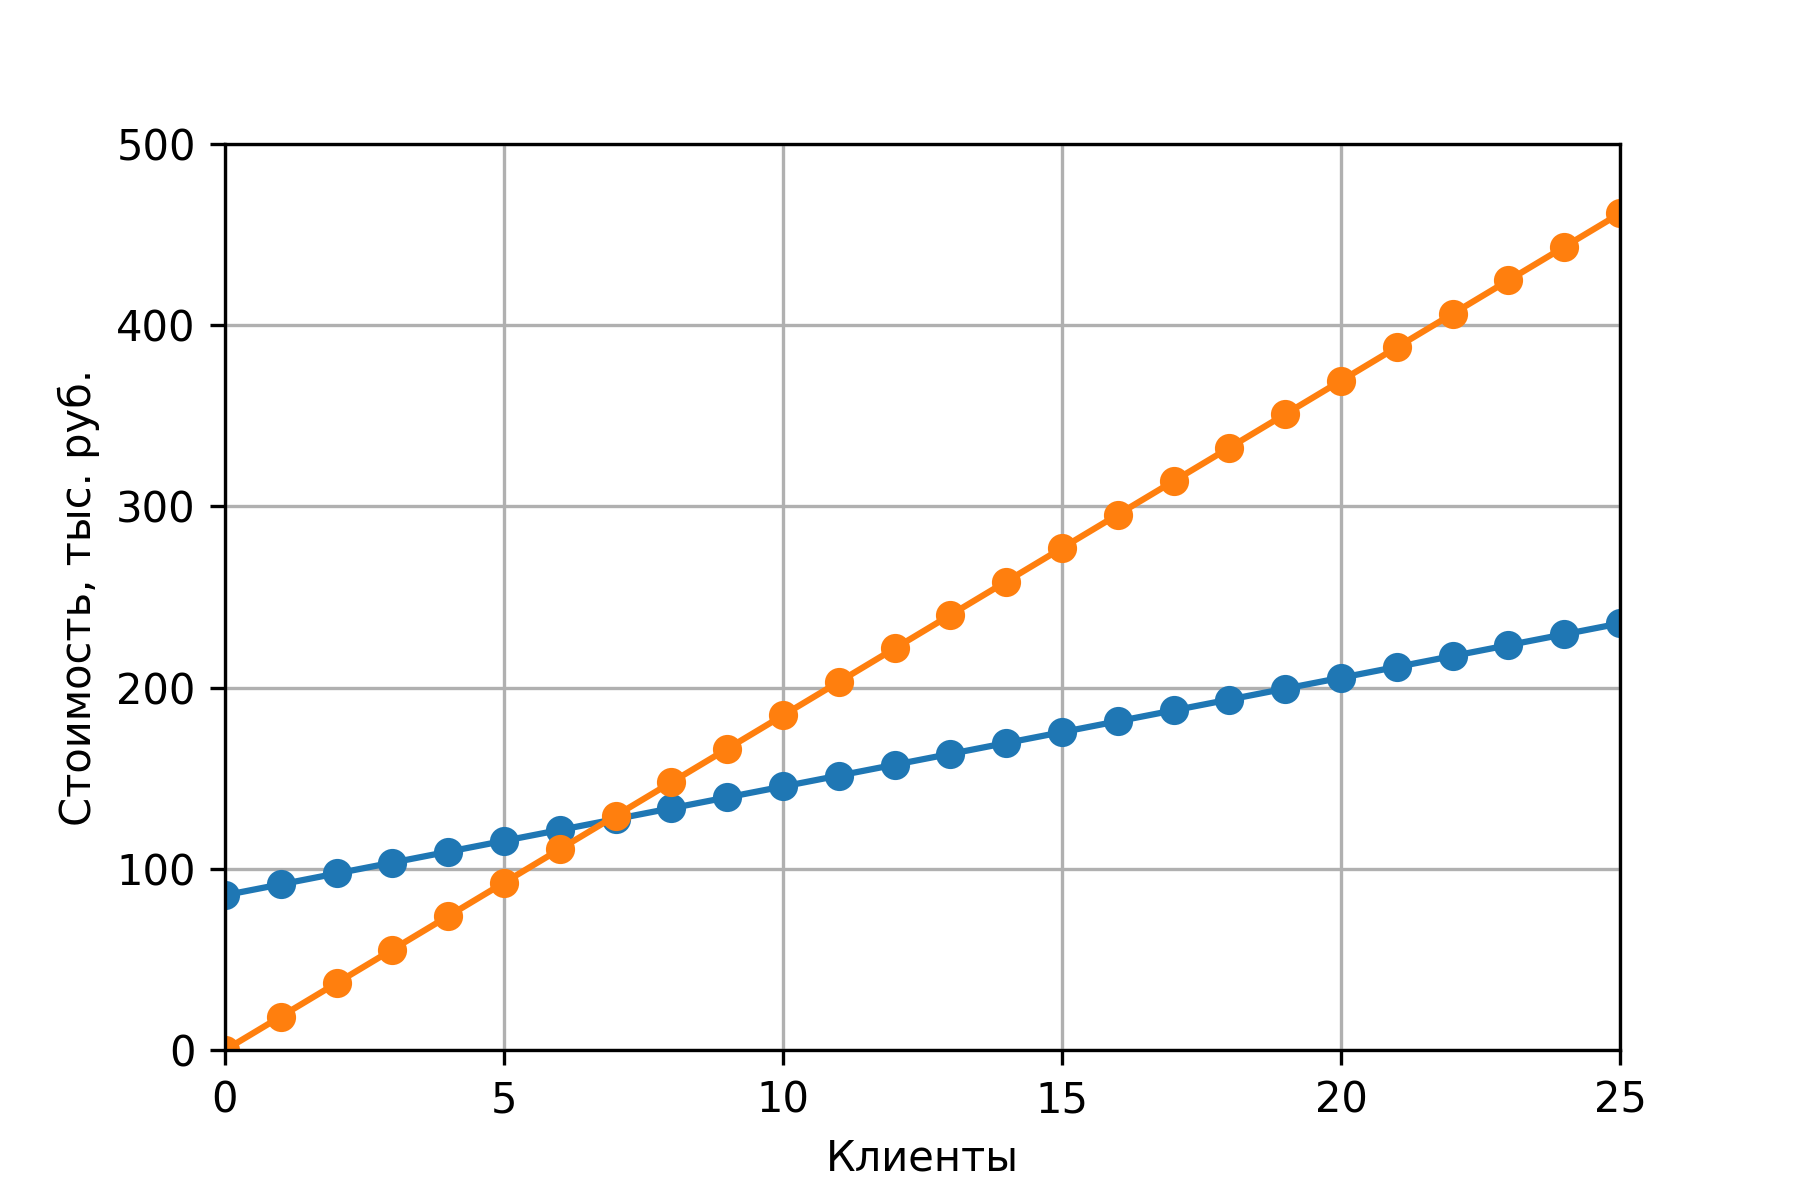
\includegraphics[width=\linewidth]{price_chart}
    \caption{Зависимость стоимости системы от количества клиентов}
    \label{pic:price_chart}
\end{figure}

\begin{table}[b]
    \centering
    \caption{Стоимость комплектующих сервера}
    \label{tab:server_price}
    \begin{tabu}to \linewidth{X[m]X[2.2,c,m]X[r,m]}
        \toprule
        Компонент & Название & Стоимость, руб \\
        \midrule
        Процессор          & AMD Ryzen 5 2600                          & 8 980  \\
        Материнская плата  & Asus PRIME X370-PRO                       & 12 590 \\
        Оперативная память & Patriot Signature 16GB PSD416G26662, 2 шт & 9 998   \\
        Видеокарта         & Sapphire Radeon RX 580 PULSE 8GB          & 16 138  \\
        Накопитель         & Samsung 860 EVO 500 ГБ                    & 6 060  \\
        Блок питания       & Be quiet! Straight Power 11 850 Вт        & 14 503 \\
        \midrule
        Итог & & 68 269 \\
        \bottomrule
    \end{tabu}
\end{table}

\begin{table}[t]
    \centering
    \caption{Стоимость комплектующих рабочего ПК}
    \label{tab:pc_price}
    \begin{tabu}to \linewidth{X[m]X[2.2,c,m]X[r,m]}
        \toprule
        Компонент & Название & Стоимость, руб \\
        \midrule
        Процессор          & Intel Core i3-9100F            & 5 721 \\
        Материнская плата  & Asus PRIME B360M-A             & 5 893 \\
        Оперативная память & Crucial Value 4Gb CT4G4DFS824A & 1 331 \\
        Видеокарта         & Интегрированная в процессор    & —     \\
        Накопитель         & Kingston A400 120 ГБ           & 1 960 \\
        Блок питания       & FSP ATX-500PNR                 & 2 366 \\
        \midrule
        Итог & & 17 271 \\
        \bottomrule
    \end{tabu}
\end{table}

\fixme{Анализ на устойчивость}


\addcontentsline{toc}{chapter}{Заключение}
\chapter*{Заключение}




\printbibliography[
    heading=bibintoc
]

\addcontentsline{toc}{chapter}{Приложение А}
\chapter*{Приложение А}




\end{document}
